
\section{Aufbau}
\label{sec:assembly}
\setauthor{Quirin Ecker}

Folgend werden alle Gegenstände und Geräte für den Aufbau in Abb.~\ref{fig:assembly} angeführt.

\begin{figure}
    \centering
    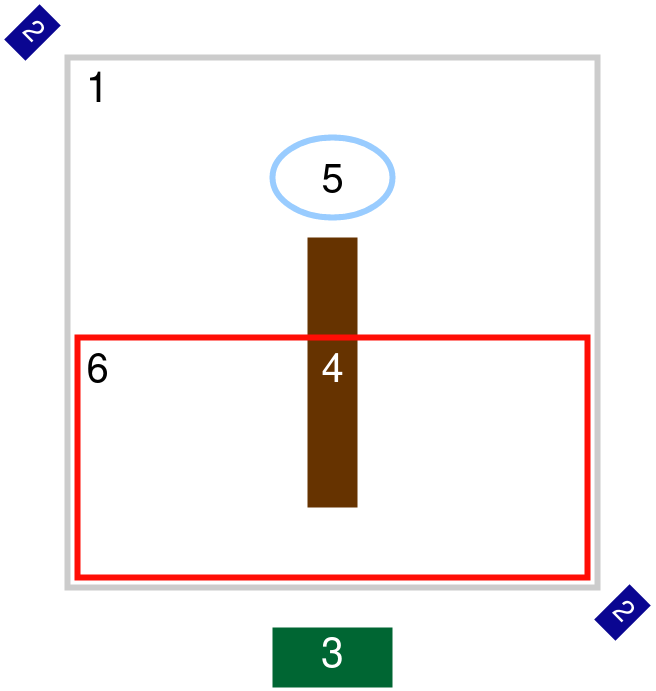
\includegraphics[scale=0.5]{pics/assemlbly}
    \caption{Aufbau}
    \label{fig:assembly}
\end{figure}

\begin{enumerate}
    \item VR Raum
    \item Lighthouses~\ref{sec:lighthouse_tracking}
    \item Monitor
    \item Balken
    \item Startposition
    \item Virtueller Abgrund
\end{enumerate}

\subsection{Erklärung}\label{subsec:description}

Der Spieler started bei der Startposition und balanciert entlang des Balkens.
Die Lichtboxen müssen diagonal positioniert werden wie bereits beschrieben in dem Abschnitt~\ref{sec:lighthouse_tracking}.
Der Balken sollte ca in der Mitte positioniert werden und die langen seiten sollten möglichst parallel zu den langen seiten des VR Raums sein.

Leichte Abweichungen der optimalen position sind nicht problematisch.
Größere Abweichungen können zu unerwarteten verhalten führen.
Die echte position des Bildschirmes ist nicht wichtig.
Wichtig ist nur wo die position bei der kalibrierung eingestellt ist~\ref{fig:assembly}.
Durch das Positionieren des Monitors wird die standard Blickrichtung für SteamVR eingestellt.
Wenn der monitor Beispielsweise auf der anderen seite eingestellt wird, schaut man in die Falsche richtung in der Simulation.

\section{Code}
\label{sec:code}

\subsection{Full-Body-Tracking}
\label{sec:full-body-tracking}

Für das Full-Body-Tracking verwenden wir ein Plugin namens Final IK.
Dieses Plugin ist ein kostenpflichtiges Programm.
Für die Diplomarbeit wurde das Plugin gratis zur Verfügung gestellt.

Für die Kalibrierung des Full Body Trackings verwenden wir einen Knopf auf dem Controller.
Dieser Vorgang ist bereits in dem Abschnitt~\ref{subsec:full-body-tracking-calibration} beschrieben.

Standardmäßig wird das Full Body Tracking mit der Taste C kalibriert.
Damit die Kalibration auch in VR erfolgen kann, ist eine Taste für das kalibrieren auch auf dem Controller reserviert.
Wie bereits in dem Abschnitt~\reft{subsec:full-body-tracking-calibration} beschrieben, ist diese Taste das Trackpad des Controllers.

Um das Kalibrieren auf eine andere Taste zu stellen, werden die Daten für das Full-Body-Tracking an die Script-Komponente übergeben, die für das horchen auf die gewünschte Taste verantwortlich ist.
Mit diesen Daten wird die statische Funktion \emph{Calibrate()} der Klasse \emph{VRIKCalibrator} aufgerufen, wenn die Taste auf dem Controller gedruckt wird.
Um zu checken, ob die Taste gedrückt wird, benützen wir das SteamVR Plugin.

In Listing~\ref{lst:defining-control-objects} werden die Objekte für das Kontrollieren der Tasten zugewiesen.
Mit diesen Objekten kann mithilfe der Update-Methode auf einen Tastendruck gehorcht werden.
Das Horchen auf diese Taste ist in Listing~\ref{lst:checking-for-input} ersichtlich.

\begin{lstlisting}[language={[Sharp]C},label={lst:defining-control-objects}, caption={Zuweisung der Kontroll Objekt}]{Zuweisung der Kontroll Objekte}
private readonly SteamVR_Action_Boolean _inputAction = SteamVR_Actions.default_Teleport;
private const SteamVR_Input_Sources RightController = SteamVR_Input_Sources.RightHand;
private const SteamVR_Input_Sources LeftController = SteamVR_Input_Sources.LeftHand;
\end{lstlisting}

\begin{lstlisting}[language={[Sharp]C},label={lst:checking-for-input}, caption={Auf Nutzerinput warten}]{Auf Nutzerinput warten}
private void Update()
{
    if (_inputAction.GetStateDown(RightController) || _inputAction.GetStateDown(LeftController))
    {
        // Calibrate();
        ...
    }
}
\end{lstlisting}

Wie bereits beschrieben werden die Daten der Script-Komponente übergeben.
Das Object welches diese Daten hält ist von dem Typen \emph{VRIKCalibrationController}.
Dieses wird schlussendlich wie in Listing~\ref{lst:vrik-calibration} verwendet.

\begin{lstlisting}[language={[Sharp]C},label={lst:vrik-calibration}, caption={Kalibrierung}]{Kalibrierung}
_calibrationControllerObject.data = VRIKCalibrator.Calibrate(
    _calibrationControllerObject.ik,
    _calibrationControllerObject.settings,
    _calibrationControllerObject.headTracker,
    _calibrationControllerObject.bodyTracker,
    _calibrationControllerObject.leftHandTracker,
    _calibrationControllerObject.rightHandTracker,
    _calibrationControllerObject.leftFootTracker,
    _calibrationControllerObject.rightFootTracker
);
\end{lstlisting}


\subsection{Beam Calibration}
\label{subsec:beam-calibration}

Das Kernthema dieser Arbeit ist, ein reales Objekt in die virtuelle Welt zu synchronisieren.
In dem Fall der Arbeit ist dieses Objekt wie bereits beschrieben ein Balken.

Die Beam Kalibration ist für die Synchronisation des realen Balkens mit dem virtuellen Balken zuständig.
In der Entwicklungsphase gab es sehr viele Ansätze diese Synchronisation zu implementieren.
Hier ist zwischen Grundansätzen und Implementierungsansätze zu Unterscheiden.
Im Zuge dieser arbeit beschreibt ein Grundansatz die grundlegende Strategie das Problem zu lösen und ein Implementierungsansatz die Strategie einen Grundansatz zu lösen.

\subsubsection{Grundansätze}

Folgend werden zwei dieser Grundansätze beschrieben.

\begin{itemize}
    \item Tracker Ansatz
    \item Marker Ansatz
\end{itemize}

Der Initial Ansatz dieser Arbeit war der \emph{Tracker Ansatz}.
Dieser Ansatz war eine Lösung mit den bereits in Abschnitt~\ref{sec:vive-tracker} beschriebenen Tracker.
In diesem Lösungsansatz würde ein Tracker in die Mitte des Balkens platziert werden.
Durch diesen Tracker und die Dimensionen des Balkens würde es in der Theorie möglich sein die Position und größe des Balkens zu berechnen.

Der Vorteil dieses Ansatzes wäre, dass der Balken wärend des Spielerlebnis verschiebbar ist, da die Position durch den Tracker aktualisiert werden kann.

Leider besitzt dieser Ansatz den ein oder anderen Nachteil.
Einer dieser Nachteile ist, dass die Dimensionen des Balkens beim Initial Setup gemessen werden müssen.
Weiters muss der Tracker in der mitte des Balkens befestigt werden, da durch Änderungen der Position des Trackers auch Änderungen des virtuellen Balkens auftreten.
Schlussendlich muss auch die Mitte des Balkens gefunden werden um den Tracker dort zu plazieren.

Da die Positionsänderung des Balkens während der Laufzeit in der BeamVR Applikation vernachlässigt werden kann wurde der zweite Lösungsansatz gewählt.

Der zweite und finale Ansatz ist der \emph{Marker Ansatz}.
Für die BeamVR Applikation reicht es normal aus, dass die Skalierung, Position und Orientierung einmal vor dem Erlebnis ermittelt werden.
Wie bereits beschrieben ist dadurch die dynamische Änderung des virtuellen Balken vernachlässigbar.

Für den Markenansatz wird kein zusätzlicher Tracker gebraucht.
Alles, was für diesen Ansatz wichtig ist, ist ein Controller und die restlichen VR Geräte.

Das Prinzip diesem Ansatz ist, dass mit dem Controller die Ecken des Balkens markiert werden.
Diese Markierungen werden von der Applikation gespeichert und später in der Game-Szene verwendet, um den Balken richtig zu positionieren, skalieren und orientieren.
Da die Höhe durch das SteamVR Setup bekannt ist, müssen nur die oberen Ecken des Balkens.

\begin{figure}
    \centering
    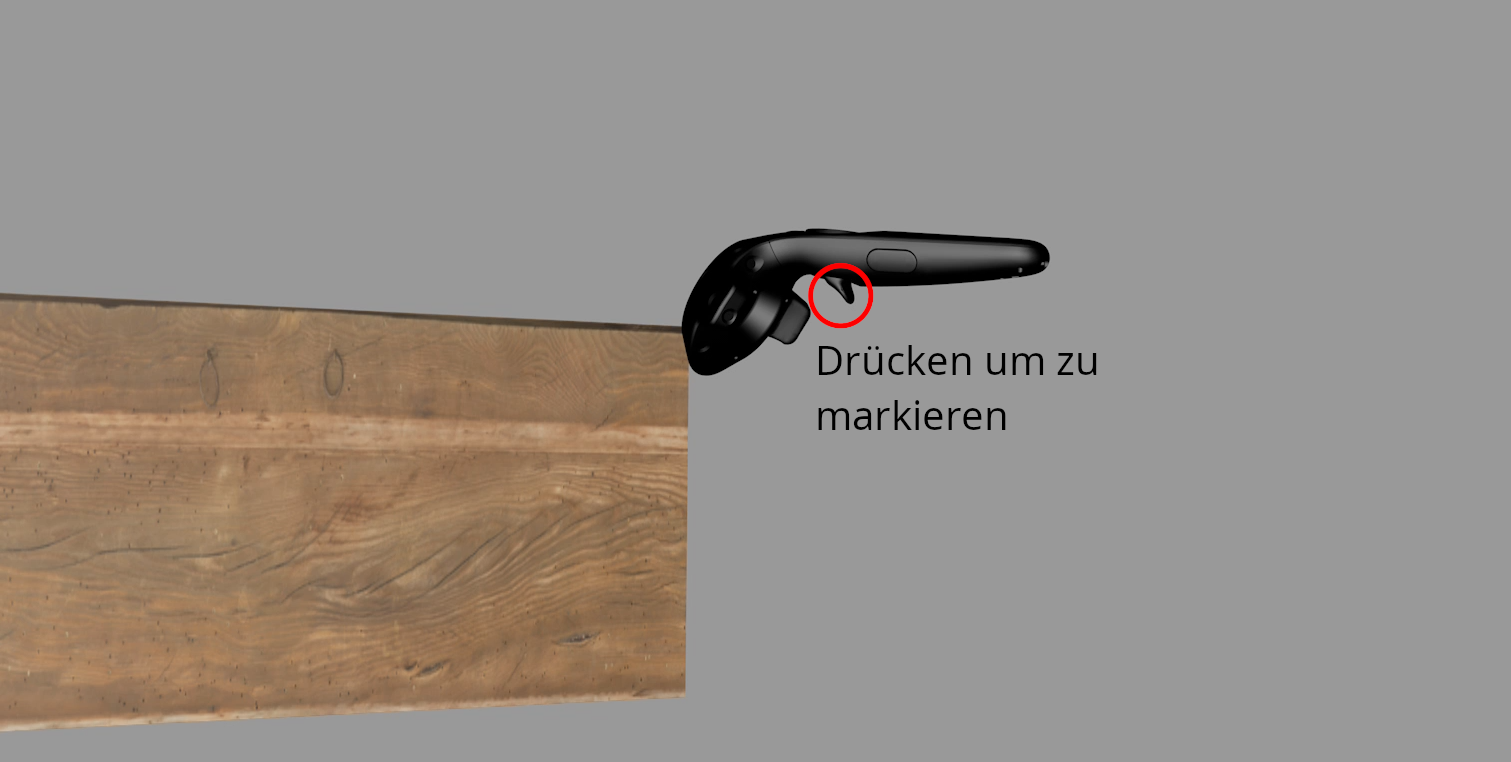
\includegraphics[scale=0.3]{pics/beam_mark}
    \caption{Markierung Einer Ecke des Balkens}
    \label{fig:beam-mark}
\end{figure}

Eine dieser Markierung wird folgendermaßen durchgeführt.
Das runde ende des Controllers muss an der gewünschten Ecke anstoßen.
Daraufhin wird der Trigger gedrückt, welcher sich an der unteren seite des Controller befindet.
In Abb.~\ref{fig:beam-mark} ist dieser Vorgan Visualisiert visualisiert.

\begin{figure}
    \centering
    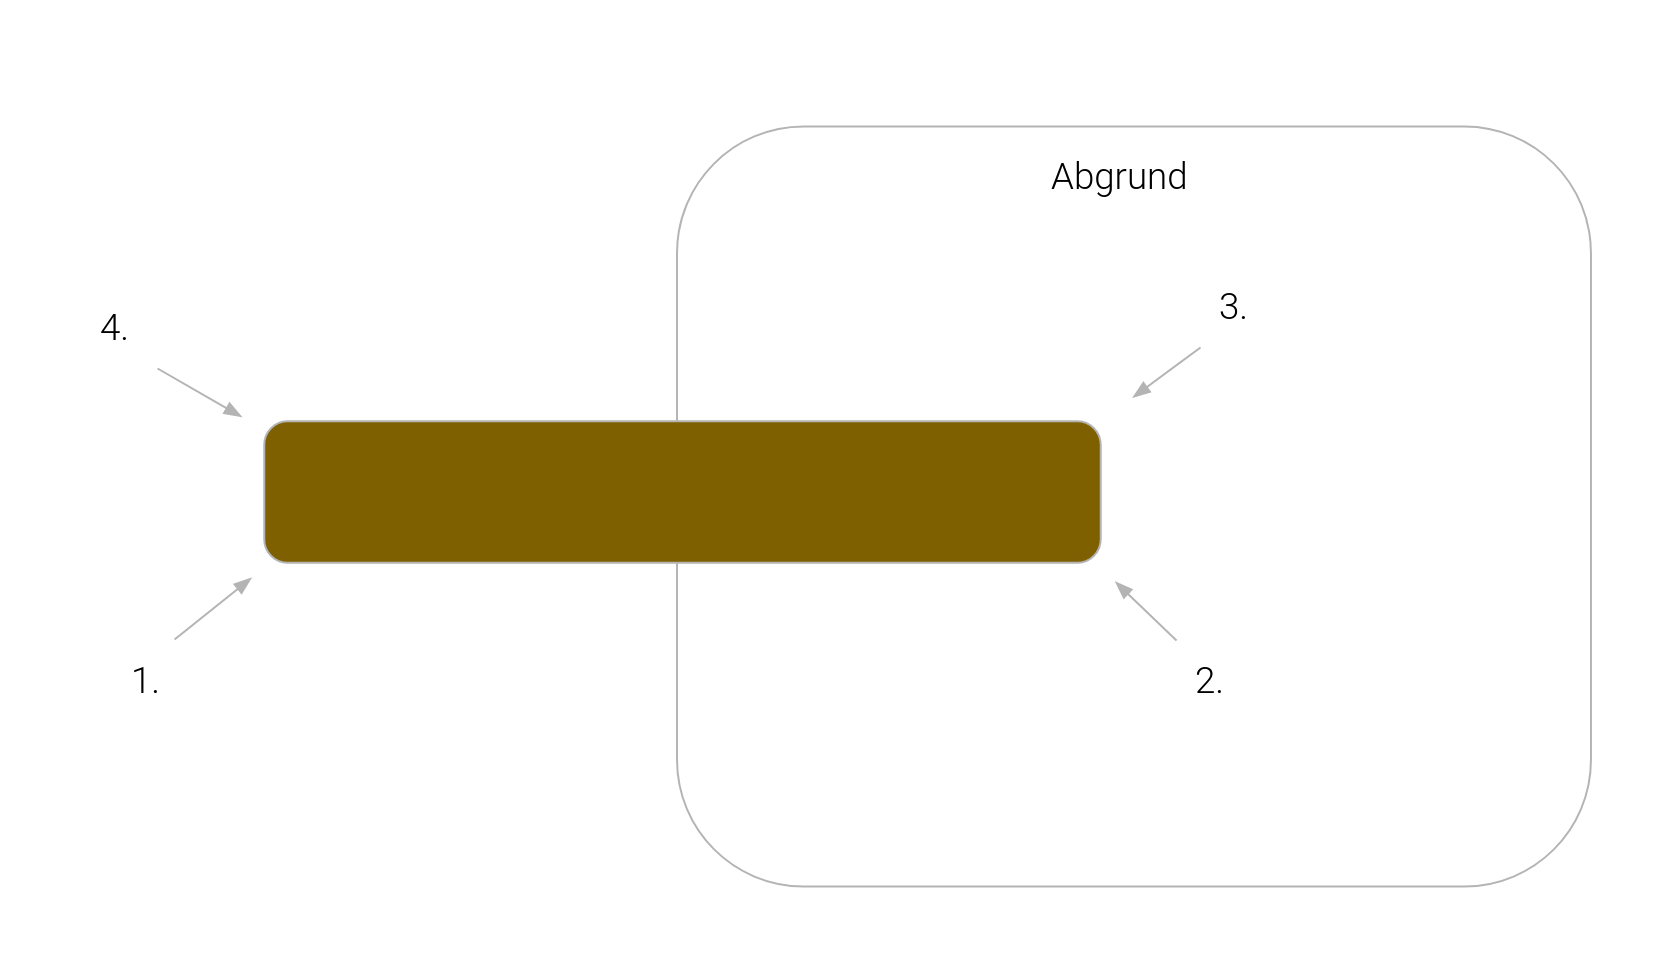
\includegraphics[scale=0.25]{pics/beam-marking-sequence}
    \caption{Reihenfolge der Markierungen}
    \label{fig:beam-marking-sequence}
\end{figure}


Für die Markierung jeder Ecke gibt es eine gewisse Reihenfolge.
Diese Reihenfolge ist von der BeamVR Applikation vordefiniert und von der Position des Abgrunds abhängig.
In Abb.~\ref{fig:beam-marking-sequence} ist die Reihenfolge ersichtlich.

\subsubsection{Implementierungsansatz}

Für den Marker Ansatz gibt es wiederum zwei verschiedene Implementierunsansätze.
Diese beinhalten:

\begin{itemize}
    \item Beam Transformation Ansatz
    \item World Transformation Ansatz
\end{itemize}

Der einfachere Ansatz ist der Beam Transformation Ansatz.
Bei diesem Ansatz passen wir den virtuellen Balken an den realen Balken an.

\begin{figure}
    \centering
    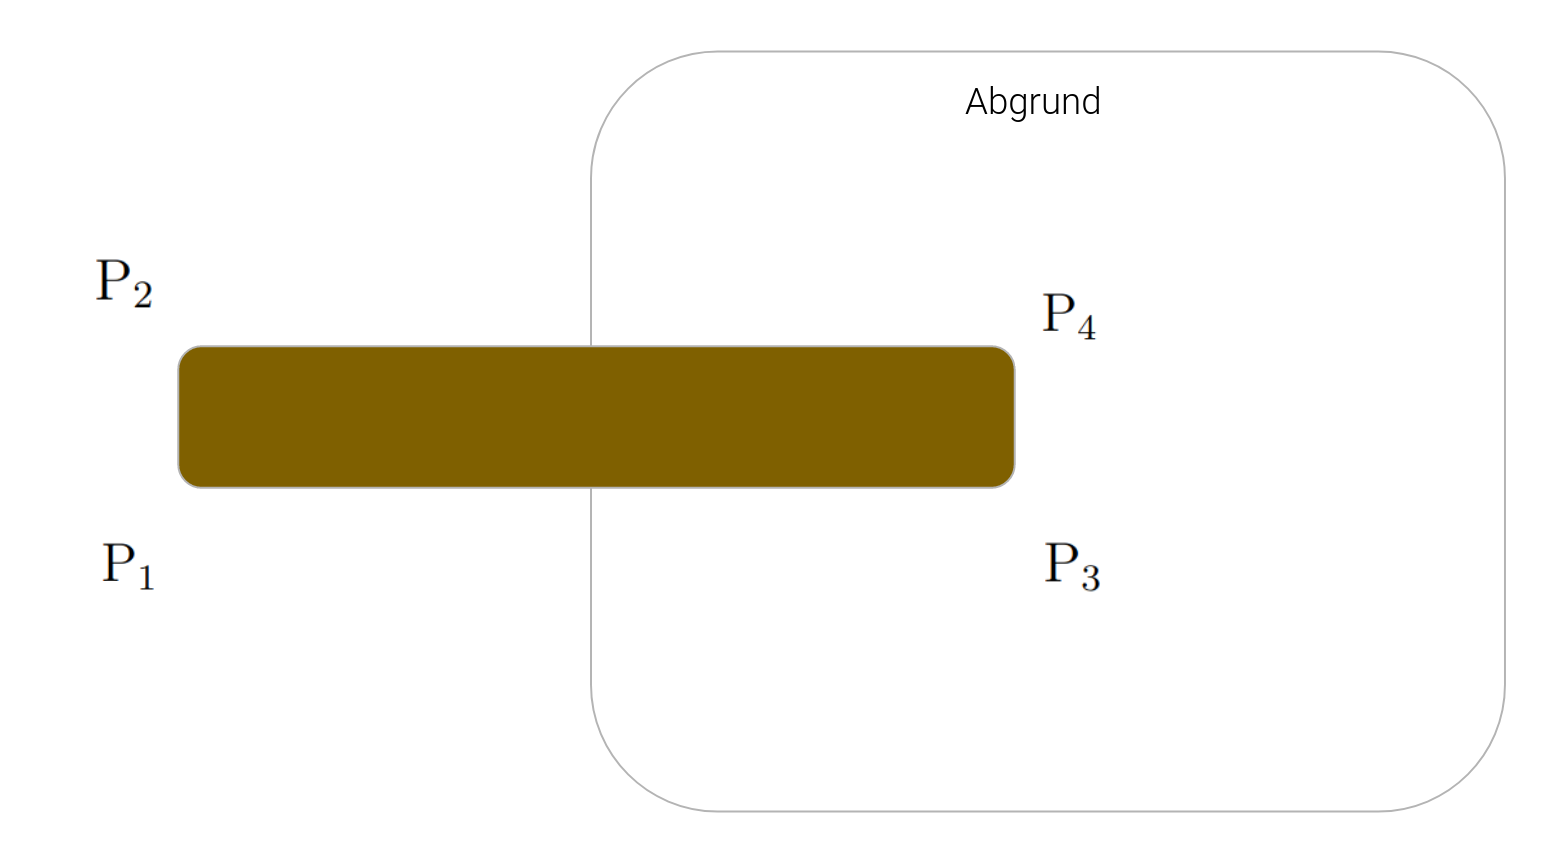
\includegraphics[scale=0.25]{pics/beam-point-labeling}
    \caption{Beschriftungen des Balkens}
    \label{fig:beam-point-labeling}
\end{figure}


Durch die Postionen der Ecken kann die Mitte berechnet werden, da davon ausgegangen werden kann, dass der Balken ein Quader ist.
In Abb.~\ref{fig:beam-point-labeling} sind die Ecken der oberen Seite des Balken mit $P_{1}, P_{2}, P_{3}, P_{4}$ beschriftet.
Die Mitte der oberen Decke kann mit folgender Formel beschrieben werden.

$$

D = (P_{4} - P_{1})

M = P_{1} +  \frac{D}{2}

$$


\subsection{Schwerkraft}
\label{subsec:gravity}

Damit die Applikation eine gewisse Spannung erhält, gibt es auch die Möglichkeit von dem Balken runterzufallen.
Dies Sollte passieren, sobald die Person auch in der physischen Realität von diesem Balken fällt.
Folgend ist die Bedingung für einen Fall und die Funktionsweise beschrieben.

\subsubsection{Bedienung}

Um ein realistisches Fallen zu gestalten ist es wichtig zu erkennen, wann eine Person nicht mehr auf den Balken ist und von dem Balek fliegt.
Die erste wichtige Bedienung ist, dass der Benutzer oder die Benutzerin über dem Abgrund ist.
Befindet sich die Person noch auf dem Haus, steht die Person zwar nicht auf dem Balken sollte aber trotzdem nicht runterfallen.

Die zweite und wahrscheinlich spannendere Bedingung ist, ab wann eine Person, welche sich über dem Abgrund befindet, von dem Balken runterfliegt.
Grundsätzlich fliegt der Benutzer oder die Benutzerin von dem Balken, wenn dieser oder diese das Gleichgewicht verliert.
Leider ist dies etwas schwierig nachzustellen, wenn sich der Balken auf dem Boden befindet.

Schlussendlich musste die Entscheidung getroffen werden, ob die Gravitation nach einem Fuß oder zwei Füßen auf dem Boden wirkt.
In der BeamVR Applikation ist die Entscheidung auf die Bediengung mit einem Fuß auf dem Boden gefallen.
Somit fällt der Benutzer die Benutzerin von dem Balken sobald ein Fuß der Person auf dem Boden ankommt.

\subsubsection{Funktionsweise}

\begin{figure}
    \centering
    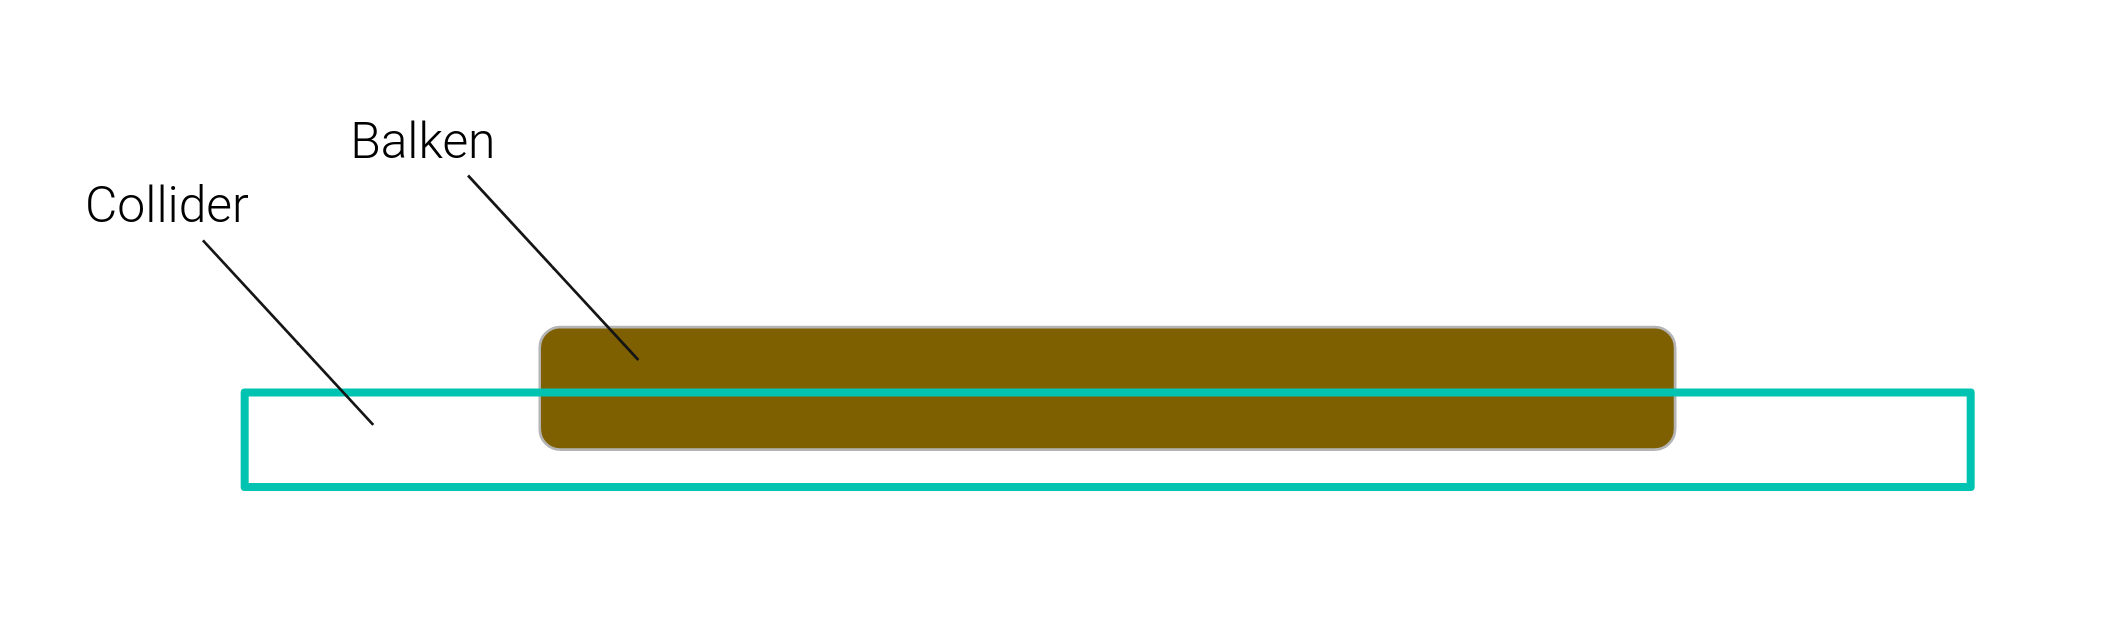
\includegraphics[scale=0.2]{pics/gravitation_collider}
    \caption{Schwerkraft Collider}
    \label{fig:gravitation-collider}
\end{figure}


Um zu checken, ob ein Fuß sich auf dem Boden befindet wurde ein Collider unter den Balken Gelegt welcher in der Höhe des Bodens ist.
Diesen Collider kann man sich wie eine Unsichtbare Box vorstellen.
In Abb.~\ref{fig:gravitation-collider} ist diese Anordnung visualisiert.

Die Höhe des Bodens wird durch das SteamVR Setup ermittelt.
Hier werden die Kontroller auf den Boden gelegt und in dem Setup auf Kalibrieren gedrückt, um die Höhe des Bodens zu ermitteln.
Dies funktioniert anhand der getrackten Controller.
Weitere Informationen über das SteamVR Setup können in Abschnitt~\ref{subsec:steam-vr-setup} gefunden werden.

Kollidiert einer der Füße mit dem Collider, wird die gesamte VR Fläche mit einer Beschleunigung von 9.81 m/s nach unten bewegt.
Kurz bevor die Fläche auf dem Boden aufkommt, wird in eine GameOver Szene gewechselt.

Um die Möglichkeit zu verhindern, dass der Kopf durch das Haus fliegt, da nur die füße sich auf dem Boden befinden und der Kopf immer noch über dem Haus wurde ein weiterer Check eingebaut.
Dieser Check beinhaltet, dass das Headset sich über dem Collider sich befinden muss, damit der Spieler oder die Spielerin runterfliegt.
Befindet sich das Headset noch über dem Haus kann der Spieler oder die Spielerin nicht von dem Haus fliegen.


\subsection{Verkehrssystem}
\label{subsec:traffic-system}
\setauthor{Florian Beckerle}
In der Stadt von BeamVR ist auf den Straßen einiges los, dass wurde mithilfe eines neuem Verkehrssystems umgesetzt.
Die Straßen sind mit, f\"ur den Spieler unsichtbaren, Objekten versehen die den Verkehr regeln.

\textbf{Car Signals}
Damit die Fahrzeuge in BeamVR wissen wo und vor allem wie sie auf den Straßen navigieren k\"onnen, wurde das Car Signal System entwickelt.
Die Car Signals gibt es in zwei verschiedenen Versionen, f\"ur die linke Straßenseite wurden gr\"une und f\"ur die Rechte Seite wurden rote Signale erstellt.
Die Signale funktionieren wie Checkpoints, jedes Auto wird nachdem es initialisiert wurde, von einem zum n\"achsten fahren.
Jeder dieser Checkpoints verweist auf den nächsten, wie in einer Liste, daher weis jedes Fahrzeug wo die momentane Zielposition ist.~\ref{fig:trafficsystem_next_signal_reference}
Endpunkte sind spezielle Signale, welche auf keinen nachfolgenden Punkt mehr verweisen, erreicht ein Auto ein solchen Punkt hat es das Ziel erreicht.

An Kreuzungen befinden sich mehrere dieser Car Signals, damit die Fahrzeuge auf der richtigen Spur bleiben und die Verkehrsregeln befolgen.
Die gr\"unen Linien zeigen die m\"oglichen Routen die das Auto fahren kann, die Pfeile visualisieren in welche Richtung gefahren werden kann.~\ref{fig:trafficsystem_crossroads}



\begin{figure}
    \centering
    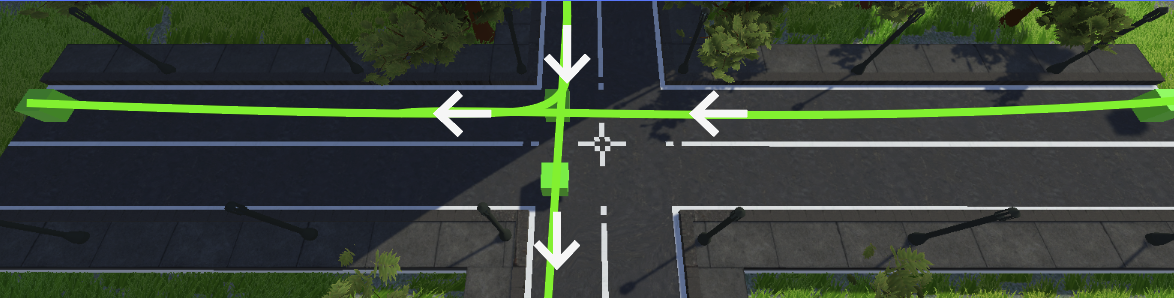
\includegraphics[scale=0.5]{pics/trafficsystem_carsignal_crossroads}
    \caption{Traffic System - Crossroads}
    \label{fig:trafficsystem_crossroads}
\end{figure}

\begin{figure}
    \centering
    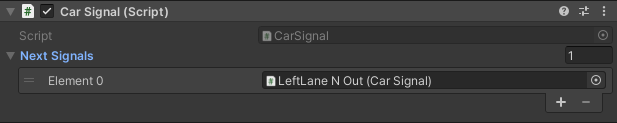
\includegraphics[scale=0.7]{pics/trafficsystem_carsignal_signal_reference}
    \caption{Traffic System - Next Signal Reference}
    \label{fig:trafficsystem_next_signal_reference}
\end{figure}


\textbf{Car Spawn Points}
Car Spawn Points sind blau dargestellte Punkte an denen Fahrzeuge, nach dem laden der Szene, initialisiert werden.~\ref{fig:trafficsystem_car_spawn_points}
Falls ein Auto einen Car Signal, welcher ein Endpunkt ist, erreicht wird es, nach einem kurzen Delay, an einem Respawn Point wieder erscheinen.
Diese Punkte verweisen, \"ahnlich wie Car Signals, auf einen nachfolgenden Punkt, wo die Fahrzeuge hinfahren.

%% IN QUELLCODEVERZEICHNIS PACKEN!
\begin{lstlisting}{CarSpawnPoint.cs}
public class CarSpawnPoint : MonoBehaviour
{

    //Location where the car should go after respawning
    public CarSignal nextSignal;

    //Position of the Respawnpoint;
    public Vector3 position;

    public void Start(){
        position = transform.position;
    }

    public Vector3 GetPosition(){
        return position;
    }

    public CarSignal GetNextSignal(){
        return nextSignal;
    }

}
\end{lstlisting}

\begin{figure}
    \centering
    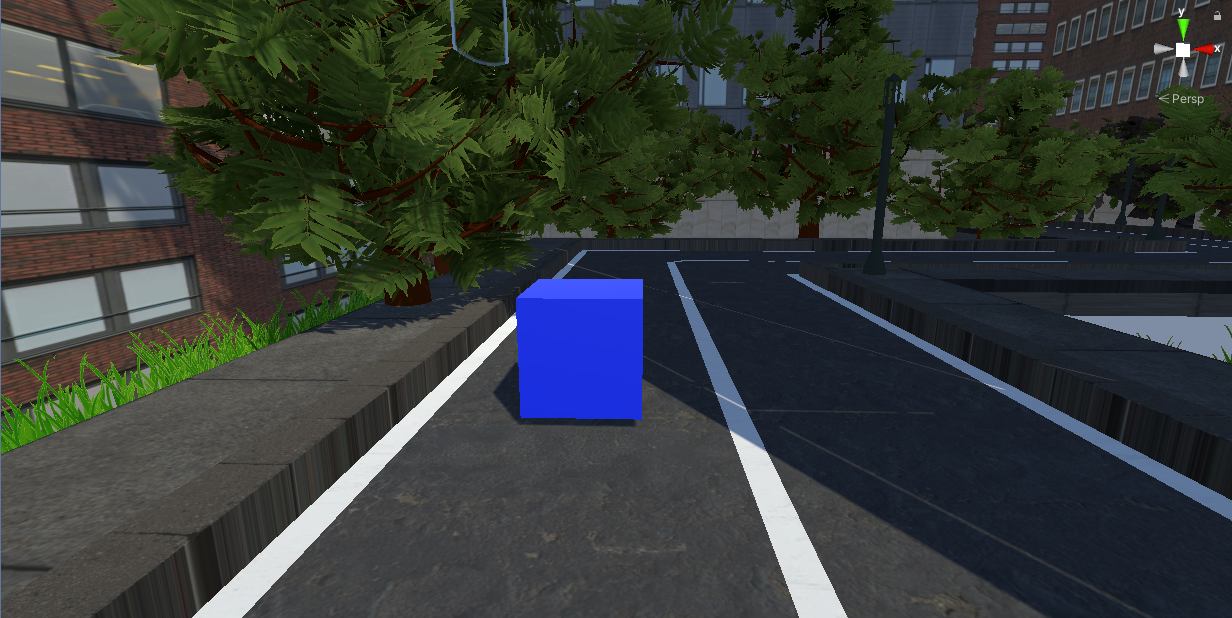
\includegraphics[scale=0.4]{pics/trafficsystem_respawn_point}
    \caption{Traffic System - Car Spawn Points}
    \label{fig:trafficsystem_car_spawn_points}
\end{figure}


\textbf{Car Manager}
Der Car Manager regelt die maximale Anzahl an Fahrzeugen die gleichzeitig auf den Straßen fahren k\"onnen.
Am Anfang werden n Fahrzeuge (n ist hierbei die maximale Anzahl an Autos) auf den Straßen initialisiert, indem ein zuf\"alliger Spawn Point ausgewählt wird.
\begin{lstlisting}{car_manager_respawncars}

public void SpawnCar(){
        CarSpawnPoint newCarSpawnPoint = GetRandomSpawnPoint();
        GameObject newCar = Instantiate(GetRandomCarModell(), newCarSpawnPoint.GetPosition(), newCarSpawnPoint.transform.rotation);
        newCar.GetComponent<CarBehaviour>().SetCarManager(this);
        CarBehaviour carBehaviour = newCar.GetComponent<CarBehaviour>();


        carBehaviour.curSignal = newCarSpawnPoint.GetNextSignal();
        carBehaviour.curPosition = newCarSpawnPoint.GetPosition();

        currentCars.Add(newCar);
    }
\end{lstlisting}

Weiters wird mithilfe der Funktion RespawnCars() ein Auto recycled, sobald es einen Endpunkt erreicht hat, indem der Manager die aktuelle Position und das n\"achste Ziel des Fahrzeuges neu setzt.
\begin{lstlisting}{car_manager_respawncars}
public void RespawnCars(GameObject finishedCar){
        CarBehaviour carBehaviour = finishedCar.GetComponent<CarBehaviour>();
        CarSpawnPoint newCarSpawnPoint = GetRandomSpawnPoint();
        carBehaviour.curSignal = newCarSpawnPoint.GetNextSignal();
        carBehaviour.curPosition = newCarSpawnPoint.GetPosition();
    }
\end{lstlisting}

\textbf{Car Behaviour}
Jedes Fahrzeug erh\"alt nachdem es initialisiert wurde eine zufällige ID mit folgendem Aufbau "Car[0-9]BeamVR[0-9]", damit diese im sp\"ateren Verlauf des Spieles besser identifiziert werden können.
In jedem Frame bewegt sich das Auto, mithilfe der Vector3.MoveTowards() Funktion, richtung dem Car signal, welches derzeit als Ziel festgelegt wurde.
Wenn nun das momentante Ziel erreicht wurde, sucht das Gefährt in dem aktuellen Punkt die Referenz auf das nächste Signal und bewegt sich dort hin.

Um zu verhindern, dass mehrere Fahrzeuge ineinander fahren,kann das Auto mithilfe eines Raycasts erkennen, was sich in einer bestimmten Distance vor sich befindet und im Notfall anhalten.

\begin{lstlisting}{car_behaviour_raycast}
...
RaycastHit hit;
         if (!Physics.Raycast(curPosition, transform.TransformDirection(Vector3.forward), out hit, carSeeingDist, layerMask))
        {
        ...
        }
...
\end{lstlisting}

\section{3d Welt}\label{sec:3d-world}
\setauthor{Florian Beckerle}
Jedes Spiel besitzt eine Spielwelt.
Babei ist es egal ob es sich um eine 3D oder 2D Applikation handelt.
Unter den Begriff Spielwelt fällt die Umgebung in welcher sich der Spieler befindet.
Es gibt hierbei so gut wie keine Einschränkungen in Bezug auf Kreativität, egal ob die digitale Welt nun ein riesiger Ring, der im Weltall schwebt,
oder eine verlassene Großstadt in einer postapokalyptischen welt, siehe Abb. ~\ref{fig:3d_environment_destiny2}.
~\cite{GamesRadar_HaloRing_2022}



%% this image and the next are not working. see issue #1

\begin{figure}
    \centering
    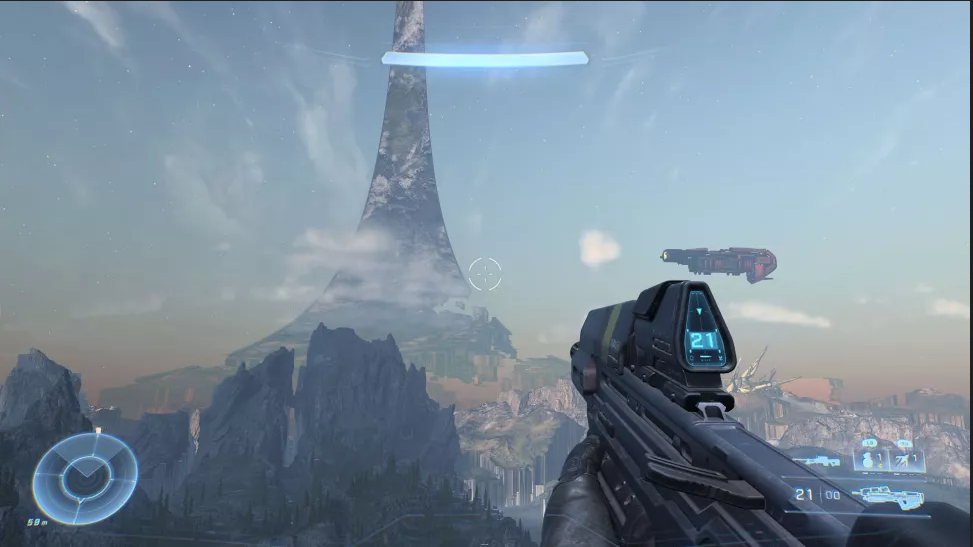
\includegraphics[scale=0.4]{pics/3d_welt_halo_ring}
    \caption{3D Welt - Halo}
    \label{fig:3d_environment_halo}
\end{figure}


%% Grafik für Destiny 2 Locations noch einbinden (Seite für Quelle lädt grade nicht Bungie.net)

\begin{figure}
    \centering
    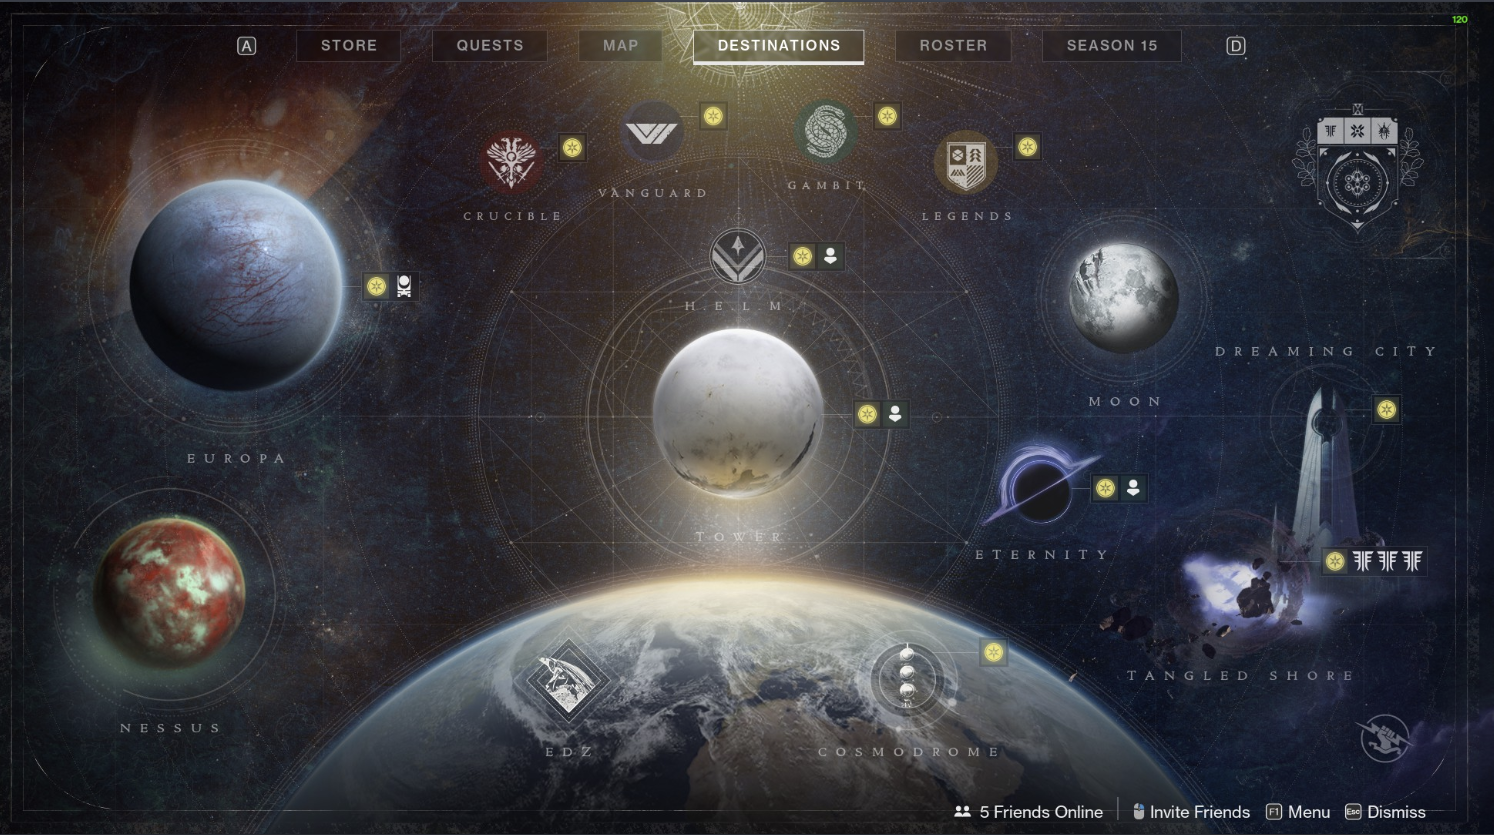
\includegraphics[scale=0.3]{pics/3d_welt_destiny_planets}
    \caption{3D Welt - Destiny 2}
    \label{fig:3d_environment_destiny2}
\end{figure}

Spielehersteller bauen die Spielwelten so auf, wie es am besten zu der Vision des Spieles passt.
Gleichzeitig wird darauf geachtet, dass sich die Umgebung nicht langweilig oder leer anfühlt.
Hierfür wird Environmental Storytelling verwendet.
Darunter versteht man das Platzieren von Gegenständen und Objekten,
welche dem Spieler eine kleine Geschichte erzählen.
Das passiert jedoch nicht über Sprache sondern einfach nur über die Platzierung und das Aussehen.
Ein Beispiel hierfür w\"are das Bild von Cayde-6 (ein Charakter aus Destiny 2), welches in einem Restaurant platziert wurde.
Cayde ist einer der drei Anführer der Vanguard, welche eine Ansammlung an Guardians (Spielern und NPC) ist und gegen das Böse kampft.
In Forsaken starb Cayde jedoch und viele trauerten um ihn, als Gedenken wurde dieses Bild aufgehangen.
~\cite{GameDeveloper_2022}

\begin {figure}
    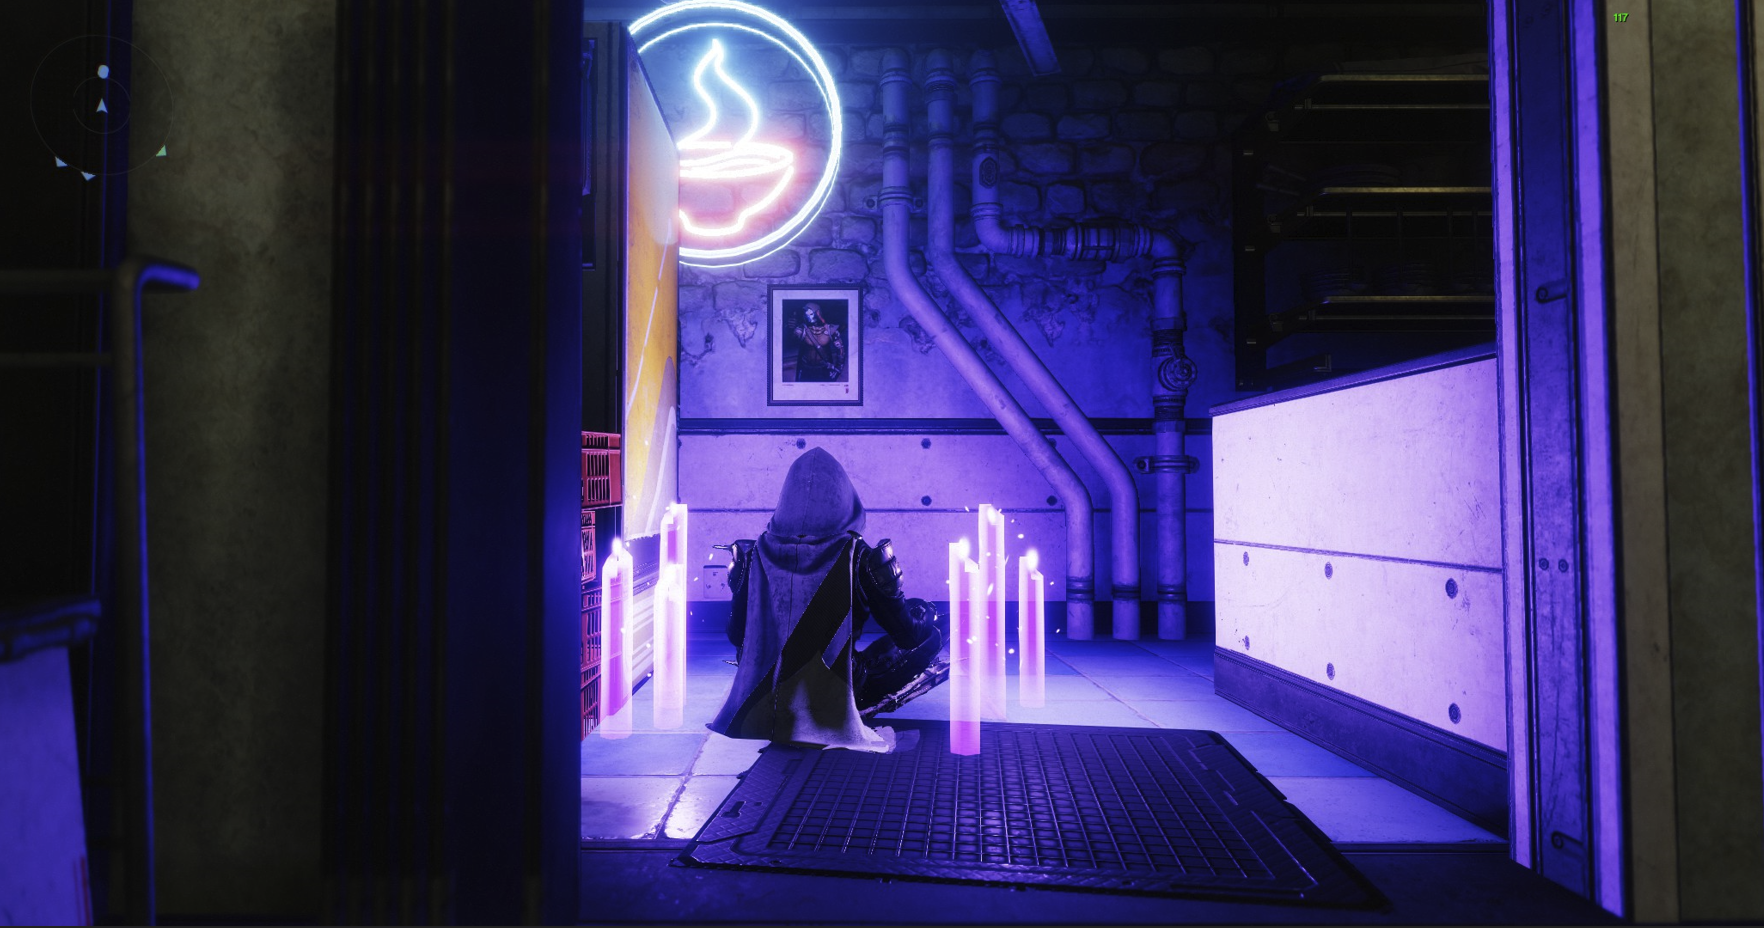
\includegraphics[scale=0.3]{pics/3d_welt_destiny2-environmental-storytelling}
    \caption{Environmental Storytelling '-' Destiny 2 Cayde}
    \label{fig:3d_environmental_storytelling_destiny2}
\end {figure}


\subsection{City Grid System}\label{subsec:city-grid-system}
\setauthor{Florian Beckerle}
Um die Gestaltung der Welt in BeamVR zu erleichtern, wurde ein Grid System verwendet.
Dafür ist die Stadt in ein Raster aufgeteilt, an welchem sich alle Objekte der Welt auf allen 3 Achsen (x,y,z) orientieren.
Unity stellt, wie in Abb. ~\ref{fig:grid-system-unity} zu sehen, so ein Grid Snapping System zur Verf\"ugung.
Daher wurde f\"ur BeamVR am Anfang der Modellierungsphase eine bestimmte Grid-Size festgelegt,
an welche die Grundfl\"achen der Geb\"aude und die Strassen
angepasst wurden.

\begin {figure}
    \centering
    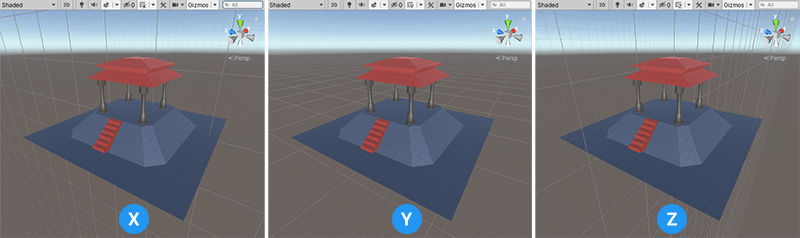
\includegraphics[scale=0.5]{pics/unity-grid-snapping}
    \caption{Unity '-' Grid Snapping System}
    \label{fig:grid-system-unity}
\end {figure}

Wenn man die Grid Size, also die Gr\"osse des Rasters \"andern m\"ochte, muss man zuerst im Editor das Grid and Snap Fenster öffnen.
Als n\"achstes findet man unter dem Bereich World Grid ein Attribut namens Size, wo man die X, Y und Z Achsen frei und unabh\"angig voneinander umskalieren kann, siehe Abb. ~\ref{fig:grid-size-unity}.
~\cite{Unity_GridSnapping_2022}

\begin {figure}
    \centering
    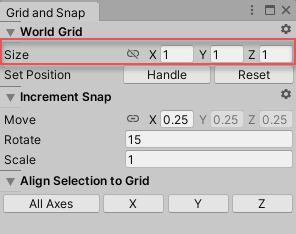
\includegraphics{pics/unity-grid-snapping-size}
    \caption{Unity - Grid Snapping Size}
    \label{fig:grid-size-unity}
\end {figure}



\subsection{Stadt}\label{subsec:city}
\setauthor{Florian Beckerle}
Jede Stadt hat viele verschiedene Strukturen wie zum Beispiel Sehensw\"urdigkeiten, Bauwerke und Einrichtungen wie Kinos, Theater oder Restaurants.
F\"ur BeamVR wurden daher insgesamt \"uber 34 Geb\"aude Modelle erstellt um eine Vielfalt in der Umgebung zu erreichen, siehe Abb. ~\ref{fig:beamvr_building-variety}.

\begin {figure}
    \centering
    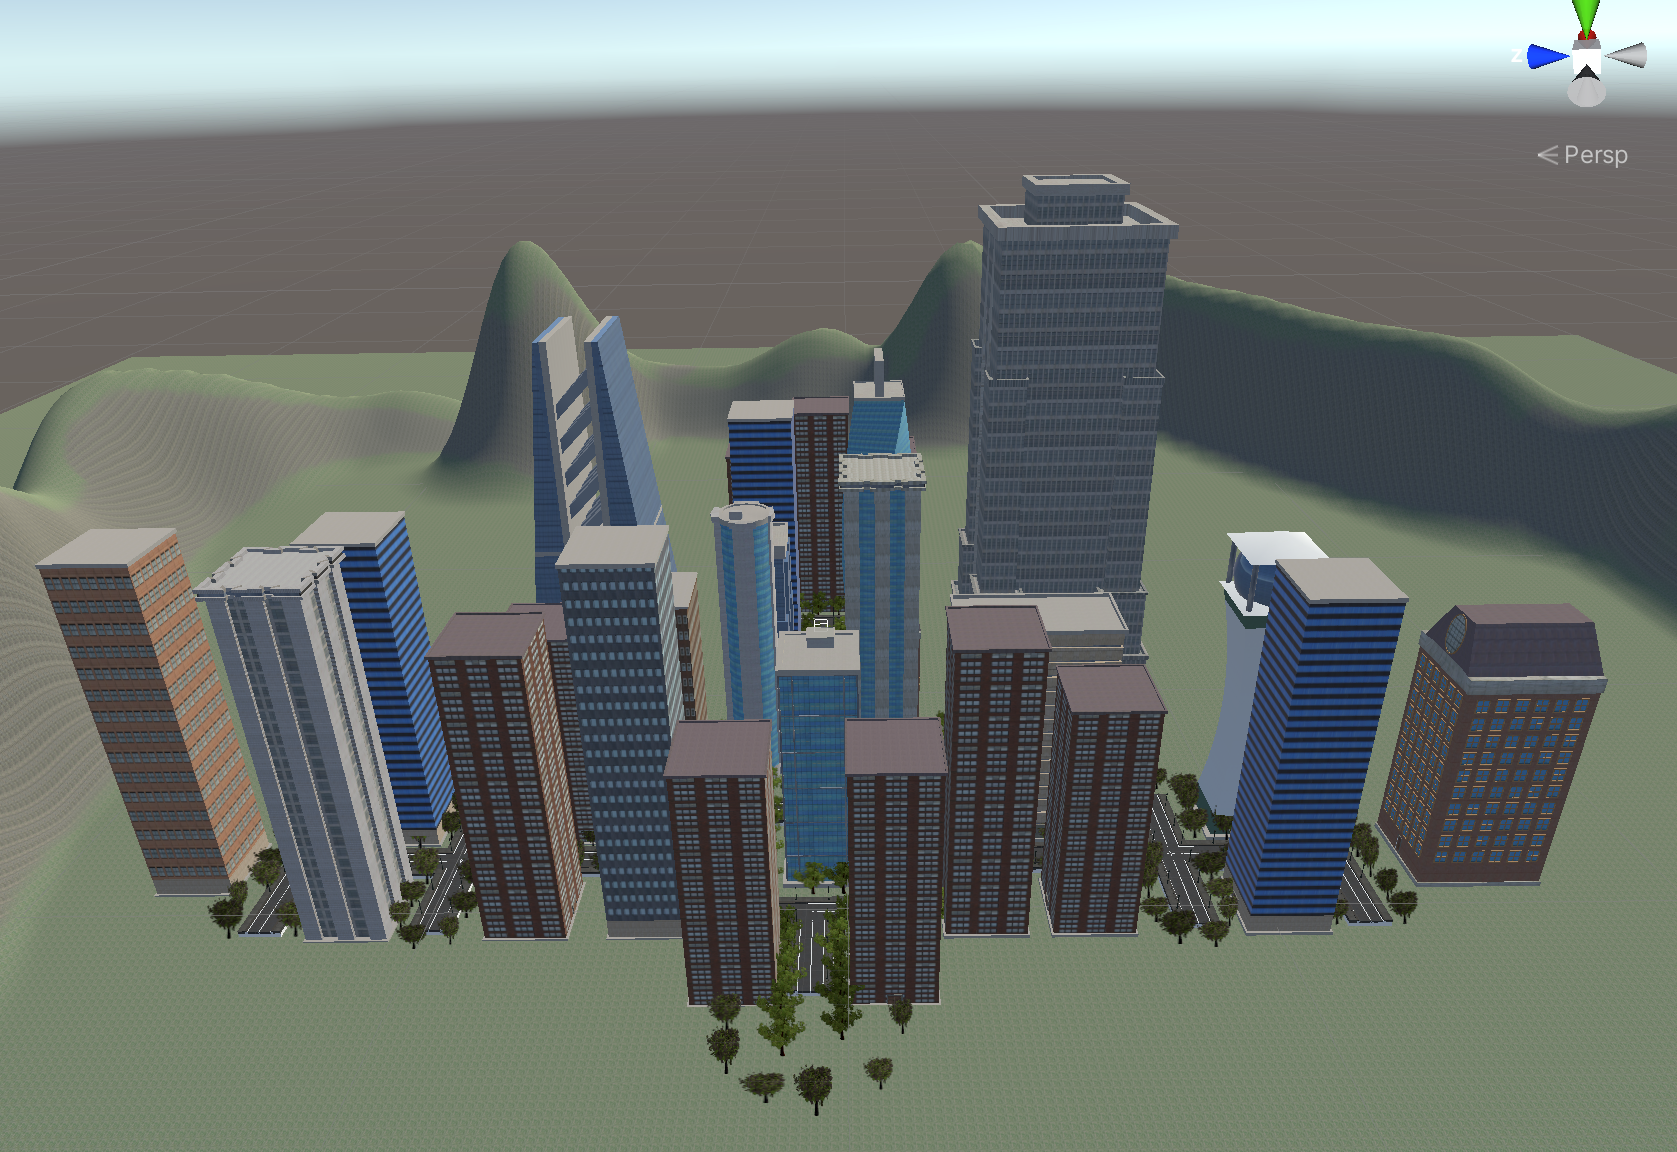
\includegraphics[scale=0.18]{pics/beamvr_building-variety}
    \caption{Beam VR - Building Overview}
    \label{fig:beamvr_building-variety}
\end {figure}

Die Stadt wurde so entworfen, dass nur die für den Spieler sichtbaren Objekte wirklich existieren, wie auf dem Abb. ~\ref{fig:beamvr_building-variety} zu erkennen ist.
Bei richtiger Umsetzung scheint es für den Anwender dennoch so, als w\"are dieser in einer kompletten Spielwelt.
Um die Performance des Spieles zu verbessern, wurde dieser Trick in BeamVR angewandt, da unn\"otige Objekte nicht gerendert oder berechnet werden m\"ussen.
Bei gr\"osseren Projekten spart das nicht nur Zeit sondern auch Ressourcen.
Bei BeamVR wurde diese Technik angewandt um die Frames per Second zu erh\"ohen.

TODO: PERFORMANCE ERHÖHEN MITHILFE VON MAPS UND TEXTUREN ERKKLÄREN!!!! (hier)


\subsection{Tag Stadt}\label{subsec:day-city}
\setauthor{Florian Beckerle}
Es wurden 17 der 34 verschieden Geb\"aude f\"ur diese Map modelliert, siehe Abb. ~\ref{fig:beamvr_building-variety}.
Der Fokus bei der Gestaltung des Bauwerke lag darauf, dass diese m\"oglichst realistisch aussehen und dennoch nicht zu rechenaufwendig in der Darstellung sind.
Daher wurden Texturen verwendet um kleinere Details an den Fassaden darzustellen, statt diese zu modellieren.
Das gleiche Prinzip wurde bei der Apocalypse Map verwendet, siehe Abschnitt ~\ref{subsec:apocalypse-city}.
Die Texturen stellen Fassaden aus Stein und Glas dar.
Ein weiterer wichtiger Punkt bei der Planung der Stadt war es auch, dass der Spieler nicht aus der Stadt raus schauen kann und die Illusion aufrecht erhalten bleibt.
Daher wurden alle umliegenden Bauwerke mindestens 3 Meter h\"oher gemacht, als das Geb\"aude auf dem sich der Spieler befindet, siehe Abb. ~\ref{fig:beamvr_building-heights}.

\begin {figure}
    \centering
    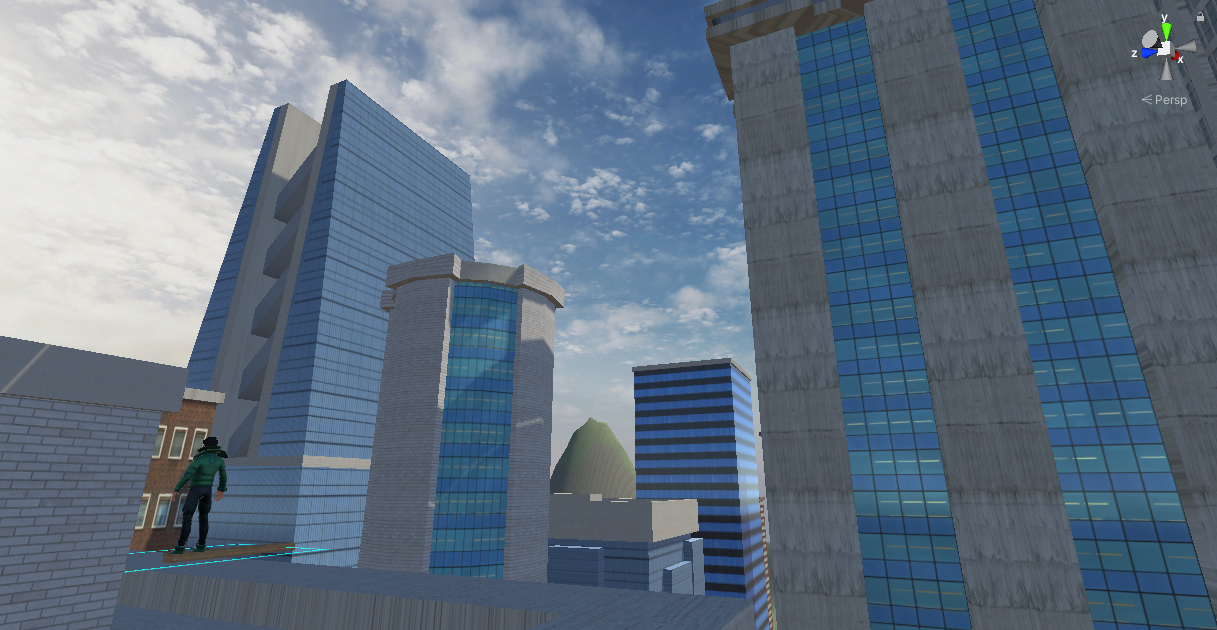
\includegraphics[scale=0.5]{pics/beamvr_city_day_heights}
    \caption{Beam VR - Building Heights}
    \label{fig:beamvr_building-heights}
\end {figure}

\subsection{Nacht Stadt}\label{subsec:night-city}
\setauthor{Florian Beckerle}
In der Nacht Version der Stadt wurde die Skybox angepasst.
Diese zeigt nun einen Sternenhimmel.
Es handelt sich hierbei um eine Sphere oder Box, welche sich um die Spielwelt befindet, sie wird dazu benutzt um einen Himmel oder andere Umgebungen,
in Form von Texturen, darstellen zu können, ohne dass diese als Modelle existieren.
Zus\"atzlich wurde die Belichtung der Scene auf ein bl\"auliches Licht eingestellt und die Laternen in den Straßen
haben noch eigene Lichtquellen.
~\ref{fig:beamvr_night_map_lighting}

\begin {figure}
    \centering
    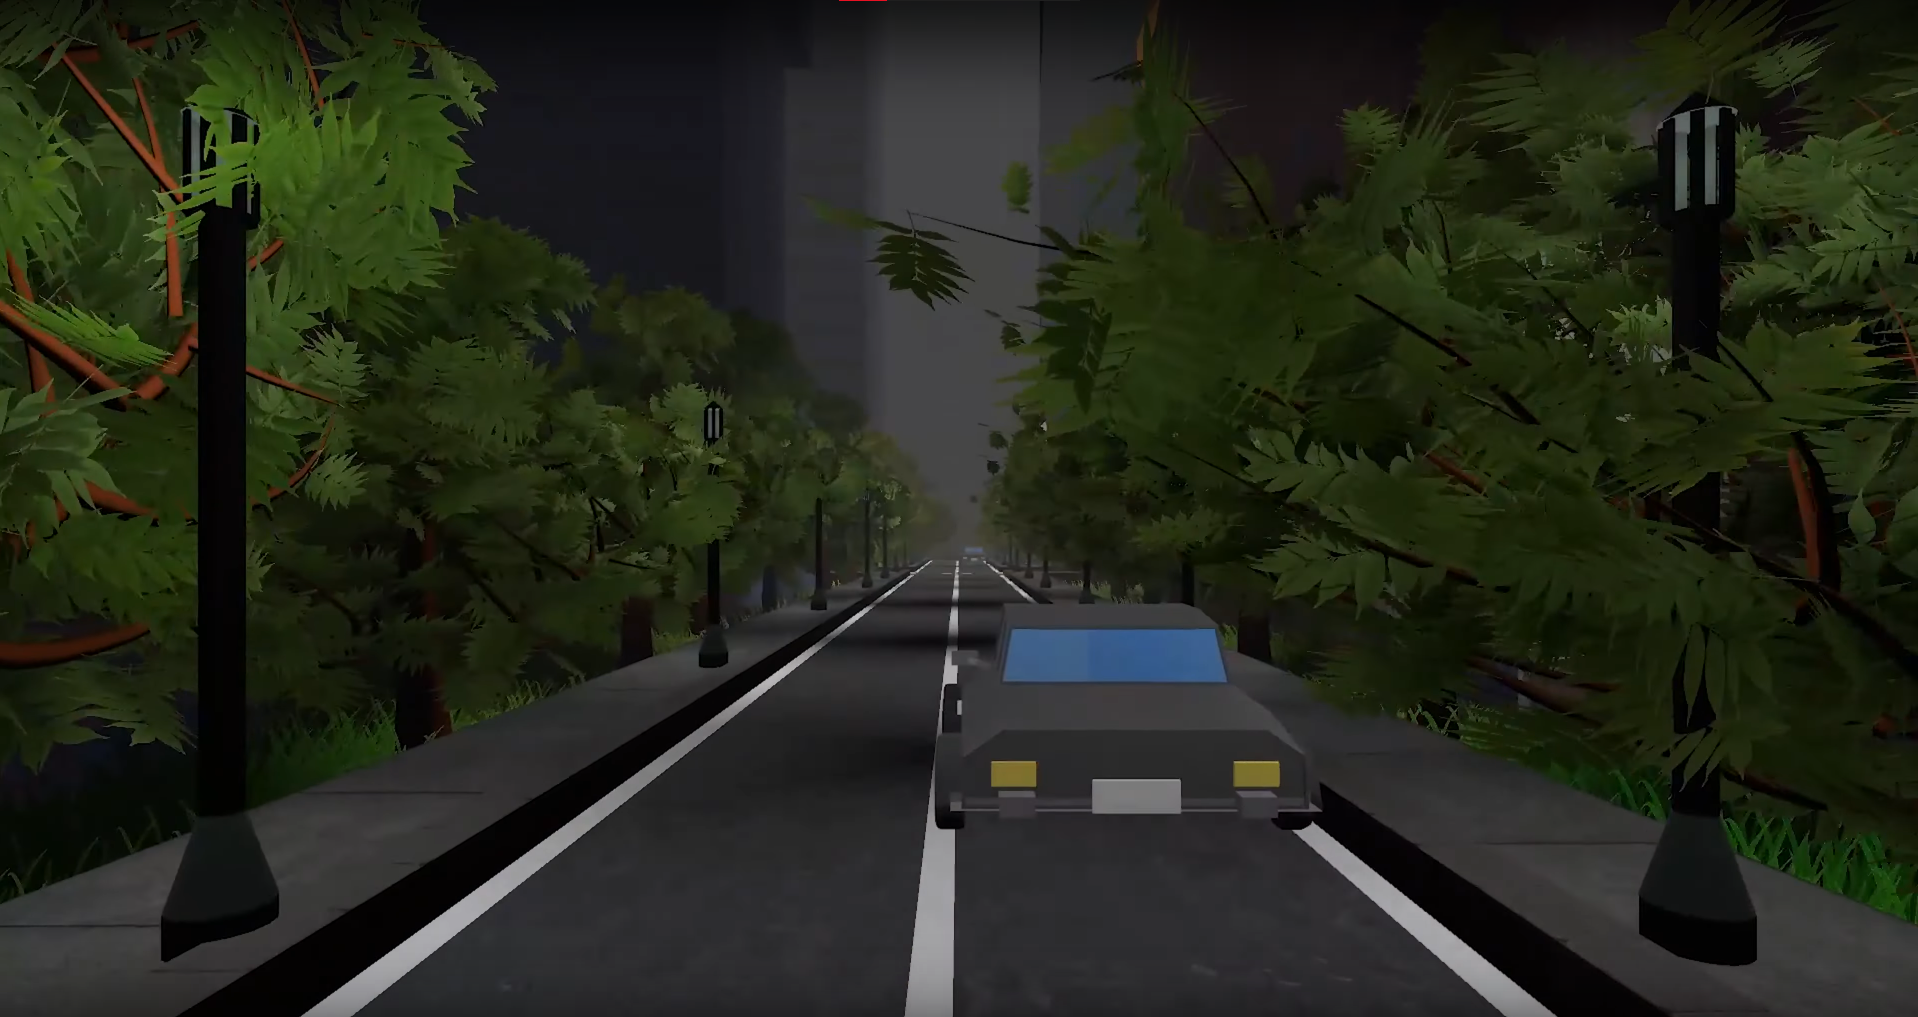
\includegraphics[scale=0.3]{pics/beamvr_night_overview}
    \caption{Beam VR - Night Map Lighting}
    \label{fig:beamvr_night_map_lighting}
\end {figure}

\subsection{Apocalypse Stadt}\label{subsec:apocalypse-city}
\setauthor{Florian Beckerle}
F\"ur diese Umgebung wurden alle Geb\"aude nochmal \"uberarbeitet.
Statt den intakten Glasfassaden werden nun vor barrikadierte Fenster und Ziegelsteine ohne Verputz f\"ur die Bauwerke verwendet, siehe Abb. ~\ref{fig:beamvr_damaged_texture}.
Durch diese \"Anderung sieht die Stadt verlassen und postapokalyptisch aus.
Um den Effekt noch zus\"atzlich zu verst\"arken wurden die Bauwerke in eine Schieflage gebracht, sodass es aussieht, als w\"urden diese gleich zusammenbrechen.
Das Gel\"ande wurde mit neuen Sandstein Texturen und D\"unen in eine W\"uste umgewandelt.
Die Planzen und B\"aume wurden durch ausgetrocknete B\"usche ausgetauscht, damit die Welt ein trostloses Aussehen erhält, siehe Abb. ~\ref{fig:beamvr_apocalypse_map}.

\begin {figure}
    \centering
    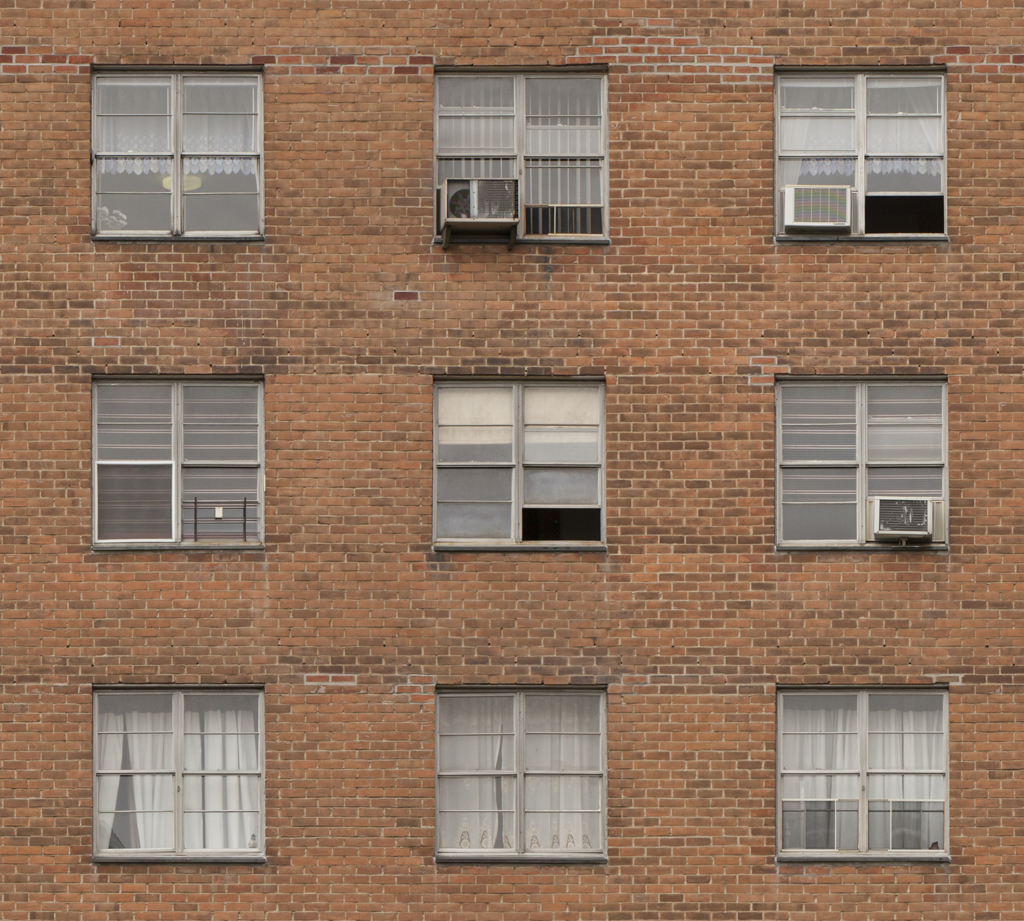
\includegraphics{pics/beamvr_damaged_texture}
    \caption{Beam VR - Damaged Texture}
    \label{fig:beamvr_damaged_texture}
\end {figure}

\begin {figure}
    \centering
    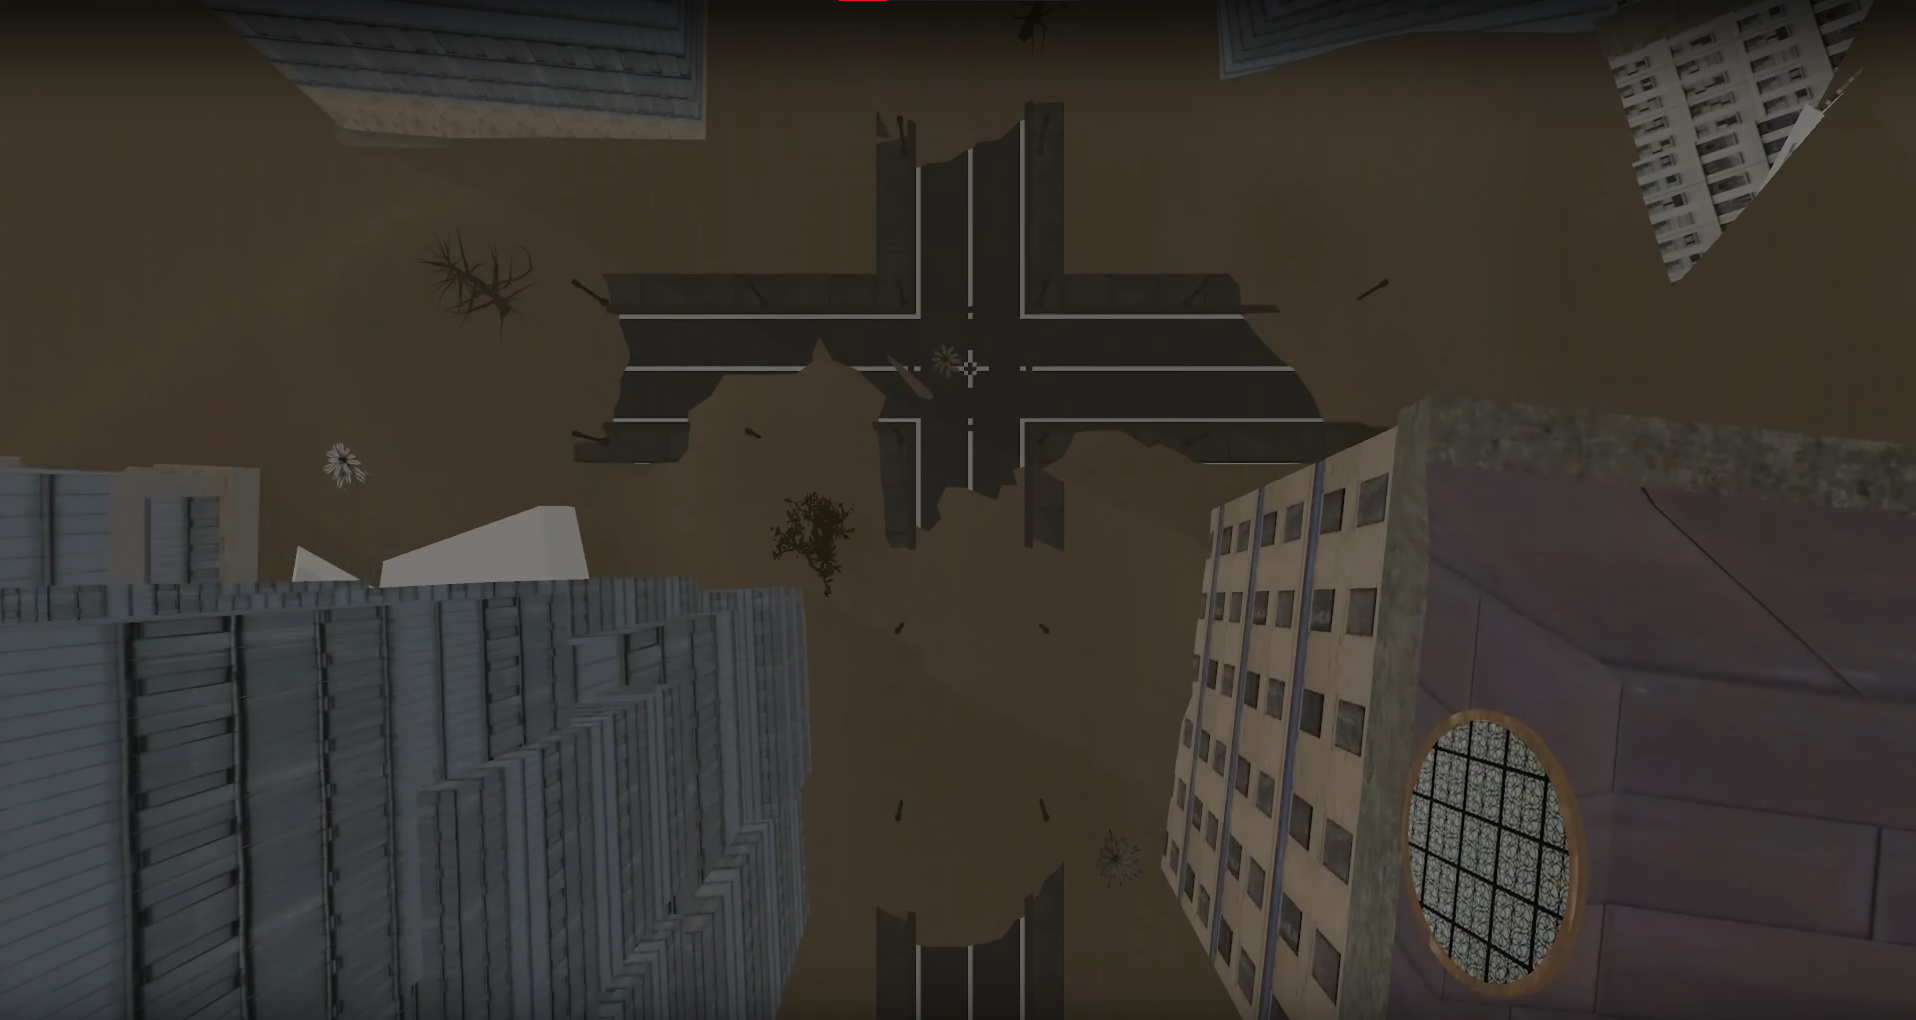
\includegraphics[scale=0.3]{pics/beamvr_apocalypse-overview}
    \caption{Beam VR - Apocalypse Map}
    \label{fig:beamvr_apocalypse_map}
\end {figure}



\section{Sound Design}\label{sec:sound}
\setauthor{Florian Beckerle}
Ohne Sound Design würden die Maps von BeamVR unrealisitsch, da in einer Stadt immer etwas los ist.
In der virtuellen Umgebung der verwendeten Game Engine existieren anfangs keine Geräusche, diese m\"ussen von den Entwicklern selber erstellt und eingef\"ugt werden.


Es gibt viele verschiedene Arten Sound Design zu benutzen, wie zum Beispiel die Ger\"ausche die der Anwender selbst in der virtuellen Welt verursacht.
Wenn sich der Spieler bewegt, sollten Fußstapfen zu h\"oren sein.
Diese klingen je nach Bodentyp unterschiedlich.
Besteht der Boden aus Holz, wird man ein h\"olzernes Klopfen und Knarren h\"oren.
Ist der Boden jedoch mit Gras bedeckt, wird ein Rascheln abgespielt.
Zus\"atzlich wird der gesteuerte Charakter außer atem sein wenn gelaufen wurde oder gerade ein Sprung ausgef\"uhrt wird, das wird mithilfe von Atem-Geräuschen umgesetzt.

Bei Umgebungen ist es wichtig, dass die Welt nicht leer klingt, sondern mit situationsbedingten Hintergrundger\"auschen voller Leben erscheint.
Es gibt jedoch auch Situationen wo gezielt wenig Umgebungsger\"ausche benutzt werden um zum Beispiel eine W\"uste oder eine verlassene Stadt noch einsamer und trostloser darzustellen.

Um die Stimmung noch genauer steuern zu k\"onnen kann Musik benutzt werden.
Wenn der Spieler auf einem Pferd durch eine Weide reitet, kann eine dramatische und inspirierende Musik benutzt werden, um den Moment noch besser und cinematischer wirken zu lassen.

Die Informationen für die Absätze wurden hier gefunden ~\cite{GK_Media_Factory_Sound_Design_2022}.

\subsection{Apocalypse}\label{subsec:apocalypse-background-sound}
\setauthor{Florian Beckerle}
Die Musik in der Apocalypse Map ist stark an das Horror Genre angelegt.
Die Melodie ist jedoch nicht wirklich existent, stattdessen existiert ein durchgehendes pfeifendes Ger\"ausch, welches unterbewusst das Spannungslevel erh\"oht.
Der Spieler f\"uhlt sich etwas unbehaglich und alleine.
Dadurch wirkt die Stadt, neben den br\"ockelnden H\"ausern, zus\"atzlich noch mehr verlassen.

Da die Sicht in dieser Map stark durch einen gelblichen Nebel, der wie ein Sandsturm wirkt, eingeschr\"ankt ist, kann man im Hintergrund den Wind pfeifen h\"oren.

\subsection{City}\label{subsec:day-night-background-sound}
\setauthor{Florian Beckerle}
Die Hintergrundger\"ausche der Tag und Nacht Version der Stadt sind sehr \"ahnlich.
Der Spieler kann Motorr\"ader und Autos auf den Straßen vorbeifahren h\"oren.
Hin und wieder kann man Menschen, die man nicht sehen kann, bei kurzen Gespr\"achen miteinander zuh\"oren und ein Kind husted im Hintergrund.

\subsection{Event}\label{subsec:building-collapse-sound}
\setauthor{Florian Beckerle}
Um spezifische Events, also bestimmte Dinge welche in der Welt passieren, f\"ur den Benutzer besser erkennbar zu machen, wurden zus\"atzlich Ge\"ausche eingef\"ugt.
Auf der Apocalypse Map sind zusammenbrechende Geb\"aude zu h\"oren, um die schlechte instandhaltung der verlassenen Stadt erneut zu verdeutlichen.
Aber wenn der Benutzer genauer hinsieht, kann man w\"ahrend diese Sounds h\"orbar sind, auch tats\"achlich eine kleine Auswahl an Bauwerken br\"ockeln sehen.

\section{Effects}\label{sec:effects}
\setauthor{Florian Beckerle}
Unity bietet verschiedene M\"oglichkeiten um das Aussehen der Applikation zu beeinflussen.
Mithilfe von Post Processing kann man Effekte zu dem Buffer der Kamera, also dem Aktuellen Frame der gerade Aufgenommen wurde, hinzuf\"ugen bevor etwas am Bildschirm Angezeigt wird.
Eine kleine Auswahl von diesen Effekten sind zum Beispiel Bloom, Grain oder Color Grading.
~\cite{Unity_Post_Processing_2022}

Post Processing kann global angewandt werden, somit werden die eingestellten Effekte \"uber die komplette Spielwelt angezeigt.
Um die Effekte auf einen bestimmten Bereich zu begrenzen muss ein Collider erstellt und platziert werden.
Wenn die Kamera in diesem Collider ist, wird das angezeigte Bild mit den eingetellten Effekten versehen.
~\cite{Unity_Post_Processing_Volumes_2022}

Der Bloom Effekt wird dazu benutzt um sehr helle Stellen und Objekte, wie bei einer echten Kamera, ausgebrannt darstellen zu können.
Hierbei wirkt das Objekt etwas verschwommen und durch die Helligkeit ist kaum etwas zu erkennen, siehe Abb. ~\ref{fig:unity-post-processing-bloom}.
\begin {figure}
    \centering
    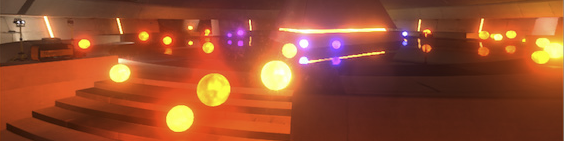
\includegraphics[scale=0.9]{pics/unity-post-processing-bloom}
    \caption{Unity - Post Processing Bloom}
    \label{fig:unity-post-processing-bloom}
\end {figure}
Dieser Effekt kann mithilfe von verschiedenen Paramtern angepasst werden.
Die Intesität steuert die stärke des Effektes, also wie stark das Bild verändert wird.
Der Treshhold filtert alle Pixel, welche unter einem bestimmten Helligkeitsniveau liegen, heraus.
Diese Pixel sind nicht von den Änderungen betroffen.
Wenn Soft Knee auf 1 gestellt wird, ist der Übergang zwischen Pixeln, die durch den Treshhold gefiltert werden, weicher.
Bei 0 befindet sich die Grenze genau auf dem eingestellten Wert.
Der Radius beeinflusst die Ausbreitung des Blooms von einem hellen Objekt aus.
Es kann zusätzlich ein Lens Dirt Effekt angewandt werden, hierbei entstehen Flecken in den Hellen stellen, siehe Abb. ~\ref{fig:unity-post-processing-lens-dirt}.
~\cite{Unity_Post_Processing_Bloom_2022}

\begin {figure}
    \centering
    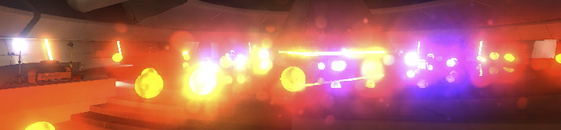
\includegraphics[scale=0.9]{pics/unity-post-processing-lens-dirt}
    \caption{Unity - Post Processing Lens Dirt}
    \label{fig:unity-post-processing-lens-dirt}
\end {figure}

Grain fügt dem angezeigten Bild einen Noise Effekt hinzu.
Hierfür wird ein nahtloses Rauschen angewandt, welches Unvollkommenheiten von Filmbändern ähnelt, siehe Abb. ~\ref{fig:unity-post-processing-grain}.
\begin {figure}
    \centering
    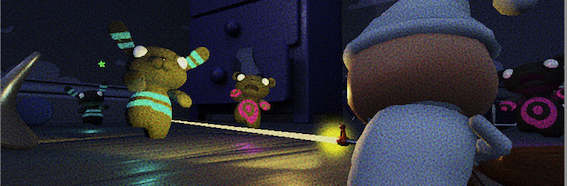
\includegraphics[scale=0.9]{pics/unity-post-processing-grain-on}
    \caption{Unity - Post Processing Grain}
    \label{fig:unity-post-processing-grain}
\end {figure}
Dieser Effekt ebenfalls mithilfe von verschiedenen Attributen verändert werden, siehe Abb. ~\ref{fig:unity-post-processing-grain-ui}.
Intensity steuert die Sichtbarkeit des Rauschen im Bild.
Luminance Contribution steuert das Rauschen abhängig von der Helligkeit einer Stelle im Bild.
Bei einem niedrigen Wert, ist in dunklen Gebieten kaum Rauschen zu sehen.
Die Größe der Partikel wird vom Size Parameter gesteuert.
\begin {figure}
    \centering
    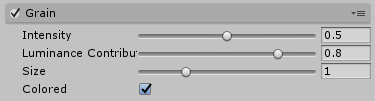
\includegraphics[scale=0.9]{pics/unity-post-processing-grain-ui}
    \caption{Unity - Post Processing Grain UI}
    \label{fig:unity-post-processing-grain-ui}
\end {figure}
~\cite{Unity_Post_Processing_Grain_2022}

Color Grading wird für die Korrektur von Farben und Helligkeit, eines Bildes verwendet.
Ein Beispiel für die Auswirkungen dieses Effekts sieht man in Abbildung ~\ref{fig:unity-post-processing-color-grading-example}.
Der Linke Teil des Bildes wurde Bearbeitet, der rechte Teil zeigt die Ursprünglichen Farben des Bildes an.
Color Grading hat 5 verschiedene Sektionen, mit welchen genauere Einstellungen getroffen werden können.
Darunter fallen Tonemapping, Basic, Channel Mixer, Trackballs und Grading Curves.
~\cite{Unity_Post_Processing_ColorGrading_2022}
\begin {figure}
    \centering
    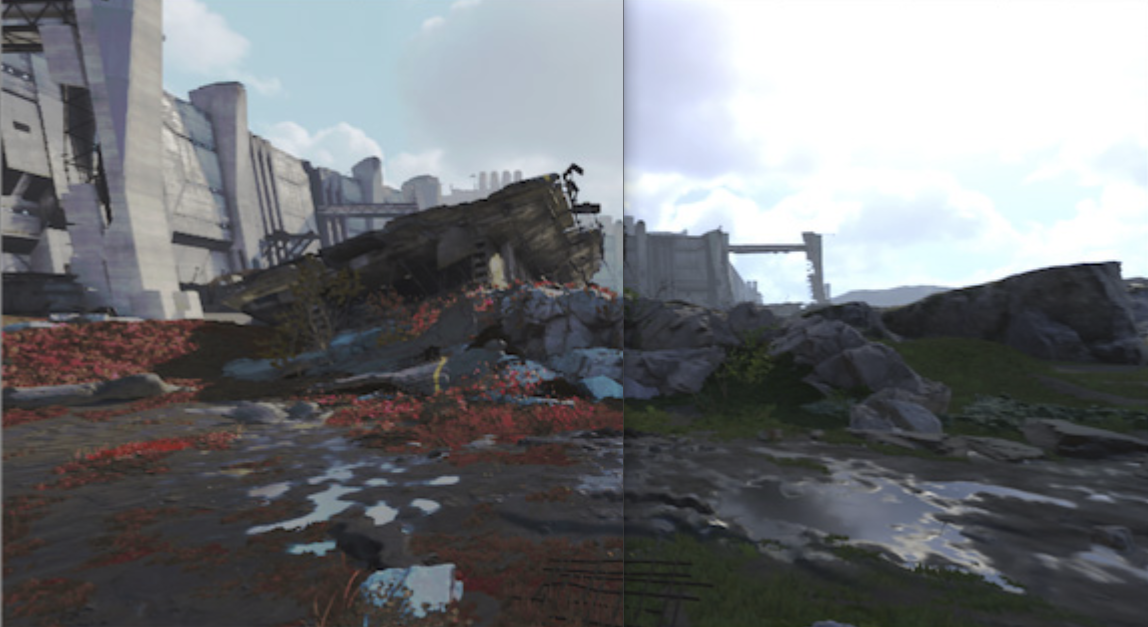
\includegraphics[scale=0.4]{pics/unity-post-processing-color-grading-before-after}
    \caption{Unity - Post Processing Color Grading Example}
    \label{fig:unity-post-processing-color-grading-example}
\end {figure}

Tonemapping beschreibt den Prozess, in welchem HDR Werte eines Bildes, so umgewandelt werden, um auf einem Bildschirm dargestellt werden zu können.
Es werden dabei drei Modes zur Verfügung gestellt.
Der Neutral Tonemaper wandelt die Werte, mit möglichst geringem Einfluss auf Farbe und Sättigung, um und verwendet eine Tonemapping Curve, siehe Abb. ~\ref{fig:unity-post-processing-neutral-tonemapper-ui}.
Black In und White In steuern dabei die inneren weißen und schwarzen Kontrolpunkten, Black Out und White Out steuern die äußeren Punkte.
Mit dem White Level kann auf einen weißen Punkt vor der Kurve eingestellt werden.
White Clip stellt auf einen weißen Punkt nach der Kurve ein.
\begin {figure}
    \centering
    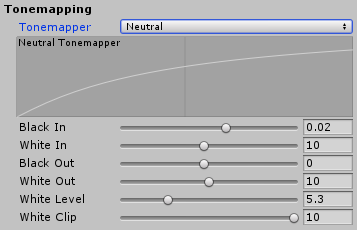
\includegraphics[scale=0.9]{pics/unity-post-processing-color-grading-neutralTonemapper}
    \caption{Unity - Post Processing Neutral Tonemapper UI}
    \label{fig:unity-post-processing-neutral-tonemapper-ui}
\end {figure}

Der Filmic (ACES) Tonemapper verwendet Schätzwerte  des ACES Tonemappers um ein filmisches Aussehen zu erreichen.
Das Resultat sind ein höherer Kontrast und es wird Einfluss auf die Farbe und Sättigung des Bildes genommen.
Dieser Tonemapper besitzt keine Einstellungsmöglichkeiten, siehe Abb. ~\ref{}.
\begin {figure}
    \centering
    
\includegraphics[scale=0.9]{pics/unity-post-processing-color-grading-filmic}
    \caption{Unity - Post Processing Filmic (ACES) Tonemapper UI}
    \label{fig:unity-post-processing-filmic-aces-tonemapper-ui}
\end {figure}

Der Basic Tonemapper stellt simple Einstellungsmöglichkeiten zur Verfügung und ist ein empfohlener Startpunkt für Farb Korrekturen.
Es können Einstellungen wie Post Exposure, Temperature, Tint, Hue Shift, Staturation und Contrast eingestellt werden, siehe Abb. ~\ref{fig:unity-post-processing-basic-tonemapper-ui}.
\begin {figure}
    \centering
    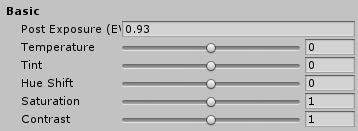
\includegraphics[scale=0.9]{pics/unity-post-processing-color-grading-basicTonemapper}
    \caption{Unity - Post Processing Basic Tonemapper UI}
    \label{fig:unity-post-processing-basic-tonemapper-ui}
\end {figure}

Post Exposure stellt die allgemeine Belichtung der Scene in EV Einheiten dar.
Dieser Effekt wird erst nach den HDR Effekten, aber vor dem Tonemapping, eingesetzt, damit die vorherigen Effekte nicht beeinflust werden.
Die Temperatur setzt die White Balance zu einer beliebig eingestellten Farbtemperatur.
Mithilfe von Tint kann ein grüner oder magenta Tint im Bild korrigiert werden.
Hue Shift verschiebt das HUE aller Farbe, während Saturation die Intensität dieser beeinflust.
Der Contrast erweitert oder verkleinert die Breite zwischen den dargestellten Farben.

Mithilfe des Channel Mixer kann der Einfluss der einzelnen Farbkanäle, welche Rot, Grün und Blau sind, auf dass gesamte Bild eingestellt werden.
Wie in Abb. ~\ref{fig:unity-post-processing-channel-mixer-ui} zu sehen ist, kann dabei jeder Farbkanal einzeln mittels eines Schiebereglers verändert werden.
Ein Beispiel für die Auswirkungen dieses Effekts ist in Abb. ~\ref{fig:unity-post-processing-channel-mixer} zu erkennen.
\begin {figure}
    \centering
    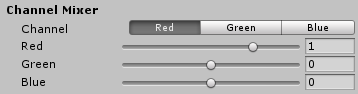
\includegraphics[scale=0.9]{pics/unity-post-processing-channel-mixer-ui}
    \caption{Unity - Post Processing Channel Mixer UI}
    \label{fig:unity-post-processing-channel-mixer-ui}
\end {figure}

\begin {figure}
    \centering
    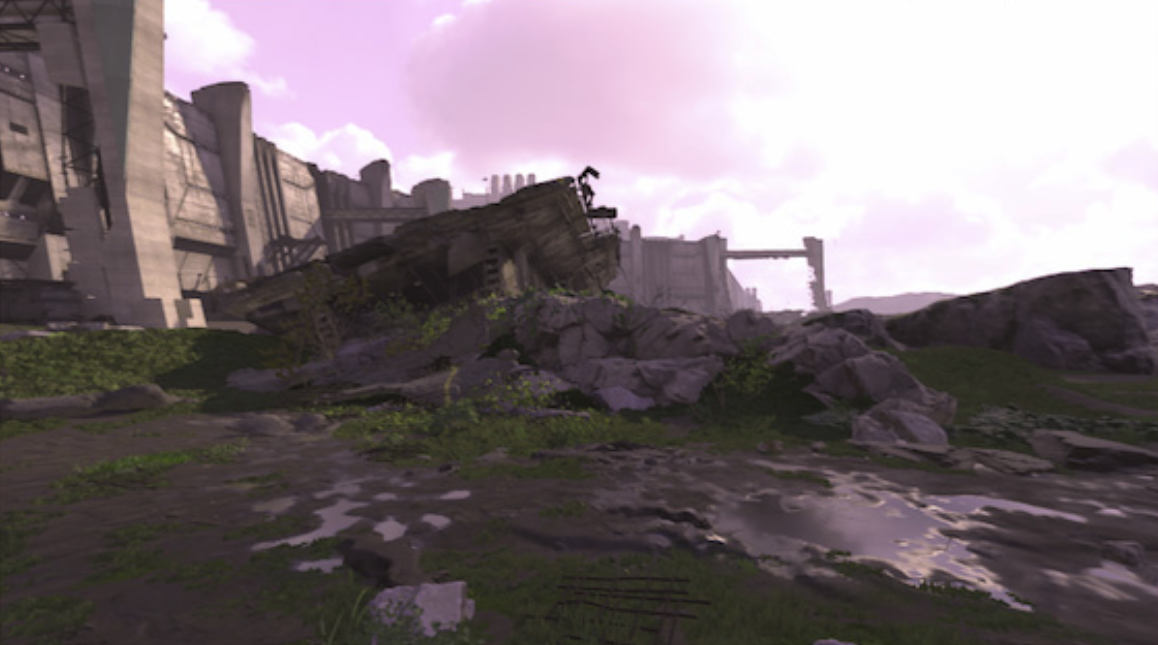
\includegraphics[scale=0.4]{pics/unity-post-processing-channel-mixer-example}
    \caption{Unity - Post Processing Channel Mixer}
    \label{fig:unity-post-processing-channel-mixer}
\end {figure}

Mithilfe von Trackballs kann man ein 3-Wege Color Grading in einem Linearen oder Logarithmischen System.
Bei der Logarithmus Variante werden die Farbverteilung und der Contrast komprimiert um einen color-timing process, welcher von optischen Film Druckern erzeugt wird zu simulieren, siehe Abb. ~\ref{fig:unity-post-processing-trackballs-log}.
Hierbei kann mit Power das Gamma und mit Offset das Signal beeinflusst werden.
\begin {figure}
    \centering
    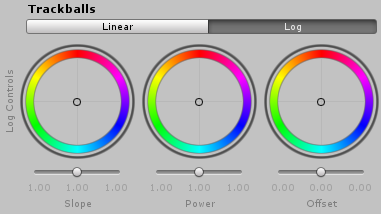
\includegraphics[scale=0.9]{pics/unity-post-processing-trackballs-log}
    \caption{Unity - Post Processing Trackballs Log}
    \label{fig:unity-post-processing-trackballs-log}
\end {figure}
Die Lineare Methode wurde für linear-encododed Data optimiert, siehe Abb. ~\ref{fig:unity-post-processing-trackballs-linear} für das UI.
Mithilfe von Lift kann das gesamte Signal verschoben werden.
Gamma beeinflusst wieder die mittleren Töne und Gain verstärkt das Signal.
\begin {figure}
    \centering
    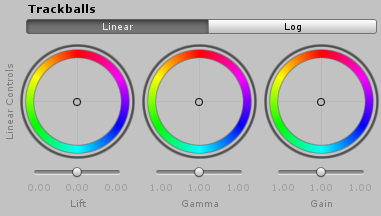
\includegraphics[scale=0.9]{pics/unity-post-processing-trackballs-linear}
    \caption{Unity - Post Processing Trackballs Linear}
    \label{fig:unity-post-processing-trackballs-linear}
\end {figure}

Mithilfe von fünf verschiedenen Grading Curves können YRGB, Hue vs Hue, Hue vs Sat, Sat vs Sat und Lum vs Sat verändert werden.
Hierbei handelt es sich jedes mal um eine Kurvendarstellung, in welcher man weitere Punkte setzen und damit den Verlauf der Kurve beeinflussen kann, siehe Abb. ~\ref{fig:unity-post-processing-grading-curve-example}.
\begin {figure}
    \centering
    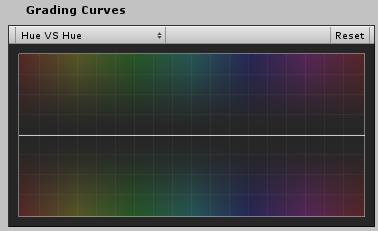
\includegraphics[scale=0.9]{pics/unity-post-processing-grading-curve-example}
    \caption{Unity - Post Processing Grading Curve Example}
    \label{fig:unity-post-processing-grading-curve-example}
\end {figure}
Bei der YRGB Kurve kann durch die Manipulation des Graphen der Contrast und die Helligkeit des Bildes eingestellt werden.
Die Hue vs Hue Kurve bietet die Möglichkeit, Farbbereiche zu verfeinern oder auszutauschen.
Um eine bestimmte Farbe besonders hervorzuheben oder einen monochromatischen Effekt zu erreichen wird die Hue vs Sat Kurve verwendet.
Bei der Sat vs Sat Kurve werden einfache Veränderungen der Farbe wie beim Color Grading vorgenommen.
Die letzte Option heißt Lum vs Sat Kurve und ermöglicht es in bestimmten Gebieten die Sättigung zu verringern, wie zum Beispiel in dunklen Stellen.

\subsection{Nebel}\label{subsec:fog-effect}
\setauthor{Florian Beckerle}
Unity bietet mehrere M\"oglichkeiten Nebel darzustellen.
Zum Beispiel mittels Post Processing, oder mithilfe der Lighting Einstellungen.
F\"ur BeamVR wurde die zweite Variante verwendet, da der Nebel in BeamVR kein Hauptaugenmerk ist und mithilfe dieser Methode das Einstellen für BeamVR schneller ging.
~\cite{Unity_Lighting_Window_2022}

Mittels Post Processing wird ein Screen-Space Nebel Effekt in der Tiefen-Texture der Kamera erstellt, siehe Abb. ~\ref{fig:unity_post_processing_fog}.
Screen-Space bedeuted, dass die Position auf dem Bildschirm und nicht in der 3 Dimensionalen Welt berechnet wird.
~\cite{Unity_Fog_2022}

\begin {figure}
    \centering
    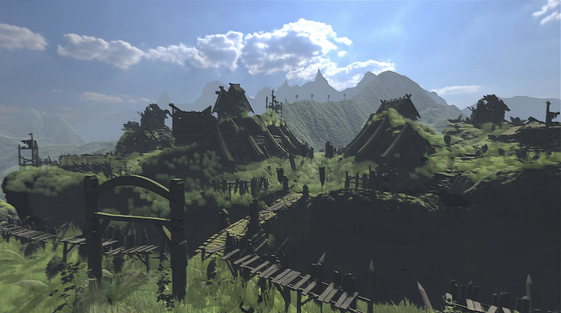
\includegraphics[scale=0.9]{pics/unity-post-processing-fog}
    \caption{Unity - Post Processing Fog}
    \label{fig:unity_post_processing_fog}
\end {figure}
Unter dem Begriff Map versteht man ein Umgebung in einer Spielwelt, in diesem Fall wird auf die Szenen, in welchen die Städte platziert sind, verwiesen.
Auf fast jeder Map von BeamVR wurde dieser Nebel verwendet.
In der Nacht Map wird mithilfe dieses Effekts ein leichter Nebel dargestellt, was zur abendlichen Stimmung beitr\"agt.
Bei Apocalypse ist der Nebel viel dichter und stellt einen Sandsturm dar. Zus\"atzlich wurde dieser gelb gef\"arbt um noch mehr an Sand zu erinnern, siehe Abb. ~\ref{fig:beamvr_yellow_fog}.

\begin {figure}
    \centering
    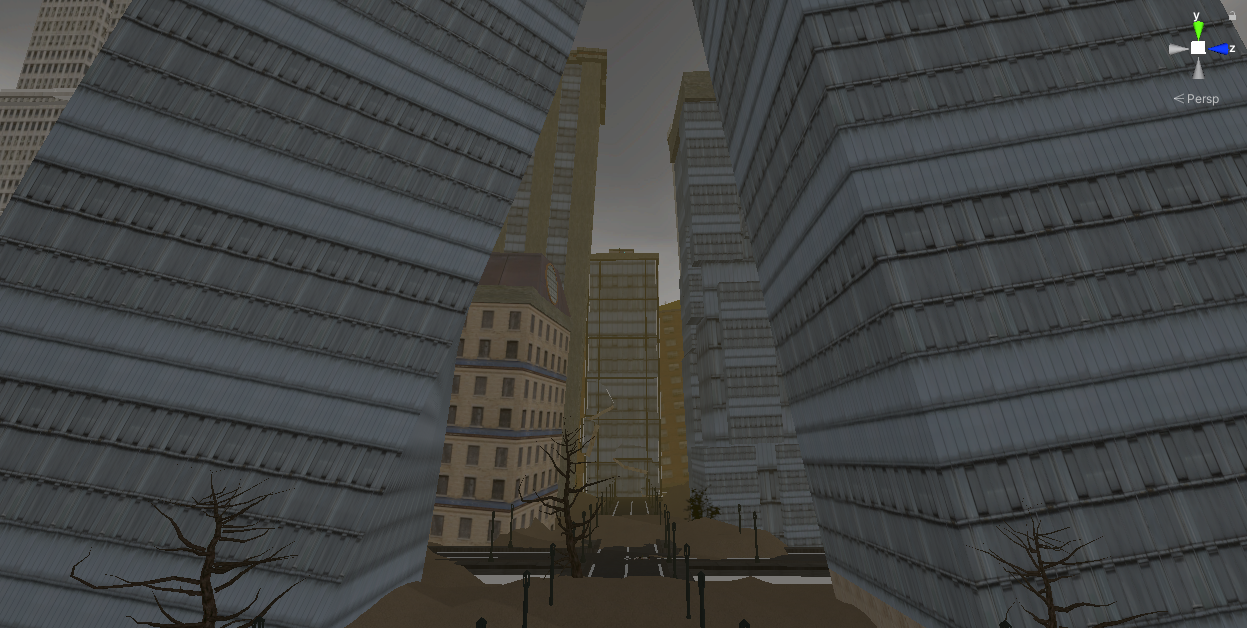
\includegraphics[scale=0.3]{pics/beamvr_yellow_fog}
    \caption{Beam VR - Yellow Fog}
    \label{fig:beamvr_yellow_fog}
\end {figure}

Mittels der High Definition Render Pipeline, welche auch als HDRP bezeichnet wird, kann ebenfalls Nebel eingestellt werden.
Hierfür wird die Volume Framework benötigt, in welcher ein Nebel Overrride hinzugefügt wird.

Diese Framework bietet einige verschiedene Optionen zur Beeinflussung des Nebels dar, siehe Abb. ~\ref{fig:unity-hdrp-fog}.
Die Option Enable wird verwendet um den Effekt zu aktivieren oder deaktivieren.
Die Fog Attenuation Distance bestimmt die Dichte und die Sichtweite im Nebel.
Ab der eingestellten Distanz, hat der Nebel bereits 63\% des Umgebungslichts absorbiert.
Dichte und Sichtweite bleiben bis zu einer definierten Base Height constant, erst ab dieser ist eine exponentielle Abnahme beider Attribute erkennbar.
Die Maximum Height und Max Fog Distance bestimmen die Stärke des Abfalls und die Distanz des Nebels.
Mittels des Color Modes kann die Farbe des Nebels beeinflusst werden.
Bei Sky Color wird die Farbe automatisch an den Himmel angepasst, während bei constant Color eine eingene Farbe eingestellt werden kann.

Volumetric Fog kann mittels der gleichnamigen Option aktiviert werden.
Die Albedo Option setzt dabei die Farbe des Nebels, mit welcher das Licht gestreut wird.
Lichter werden, mit zunehmender Dichte des Nebels, schneller abgedunkelt.
Anisotropy steuert die Streuung des Lichtes.
0 streut das Licht garnicht, 1 streut das Licht vorwärts und -1 streut rückwerts.
Mittels eines Filters kann eine Unschärfe der eingehenden Lichter geschaffen werden, damit ein weicherer Übergang zustande kommt.
~\cite{Unity_HDRP_Fog_2022}

\begin {figure}
    \centering
    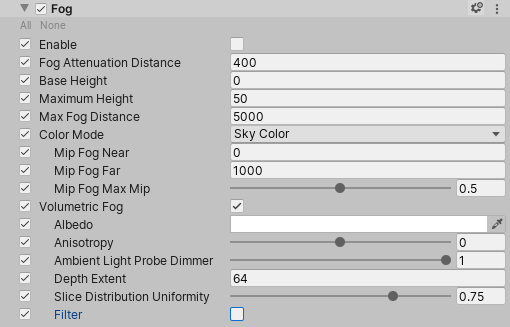
\includegraphics[scale=0.9]{pics/unity-hdrp-fog}
    \caption{Unity - HDRP Fog}
    \label{fig:unity-hdrp-fog}
\end {figure}


\subsection{Lichter}\label{subsec:light-effect}
\setauthor{Florian Beckerle}
In der Nacht Map wurden die von Unity bereitgestellten Point-Lights als Straßenlichter benutzt.
Point Lights k\"onnen mithilfe eines Radius auf einen bestimmten kreisf\"ormigen Bereich eingegrenzt werden.
Weiters wird mithilfe der Lichtst\"arke die Wirkkraft des Lichtes in diesem Gebiet genauer bestimmt.
Dank diesen Eigenschaften war das Point Light f\"ur die Aufhellung der Straßen, siehe Abb. ~\ref{fig:beamvr_street_lights}.
~\cite{Unity_PointLights_2022}
\begin {figure}
    \centering
    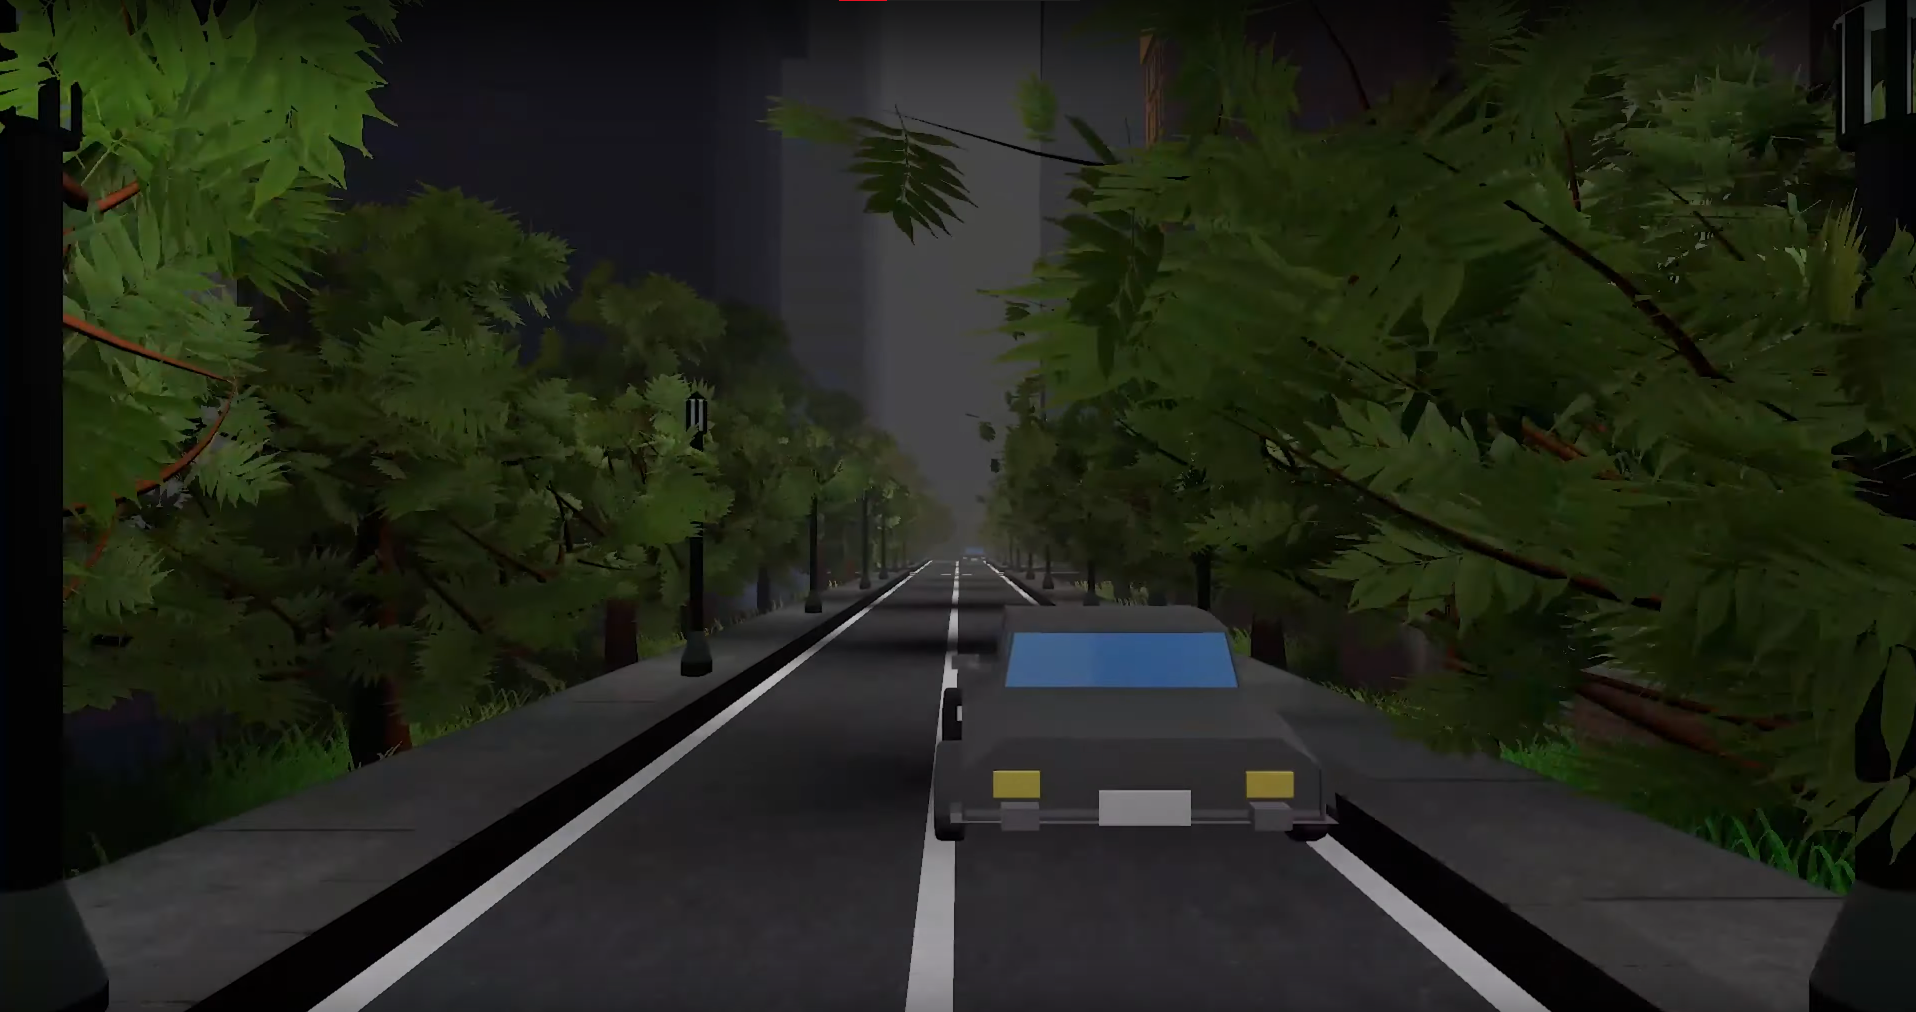
\includegraphics[scale=0.3]{pics/beamvr_point_lights}
    \caption{Beam VR - Street Lights}
    \label{fig:beamvr_street_lights}
\end {figure}


Point Lights

Spot Lights

Directional Lights

Area Lights

\subsection{Wind}\label{subsec:wind-effect}
Damit sich die B\"aume und B\"usche in BeamVR wie im Wind bewegen, werden Unitys Wind Zones ben\"otigt.
Diese Zonen sind bestimmte Bereiche, in welchen eine Windrichtung, Windst\"arke und Turbulenz definiert wird.
Die eingestellten Effekte werden dann auf alle Objekte angewandt, die mithilfe des Terrains oder Particle Systems iniziiert wurden.
~\cite{Unity_WindZones_2022}

\section{Unity Prefabs}\label{sec:prefabs}

In Unity gibt es ein System welches dem Entwickler oder der Entwicklerin erlaubt eine bestimmte Zusammenstellung von 3d Elementen zu speichern und mehrmals zu verwenden.
Wird dieses Prefab verändert verändert sich es in jeder Stelle wo es platziert worden ist.
Somit können Elemente welche aus mehreren kleineren Elementen bestehen gruppiert werden zu einem sogenannten Prefab und an mehreren Stellen verwenden.
Es werden dabei Komponenten und die Position der einzelnen Elemente relativ zu dem Prefab gespeichert.

Prefabs können auch überschrieben werden an der Stelle wo sie platziert worden sind.
Aus Erfahrung zeigt sich aber, dass dies mit Vorsicht zu genießen ist, da lokale änderungen nicht mehr global überschrieben werden.
Somit haben globale Änderungen keinen wirklichen Einfluss auf das lokale Prefab.

In der BeamVR Applikation wird dieses System an mehreren Stellen angewandt.
Beispielsweise ist es sehr nützlich, da die VR Fläche in der Applikation sich nicht wirklich abändert von Karte zu Karte.
Hier wird ein Game Prefab welches alle Game relevanten Elemente beinhaltet benutzt.
Dieses wird dann in alle Karten platziert.

Folgend wird das Game Prefab und zwei weitere wichtige Prefabs für BeamVR beschrieben.

\subsection{Game}\label{subsec:game-prefab}

Wie bereits beschrieben befinden sich alle Game relevant Elemente in dem Game Prefab.
Somit wird dieses Prefab in allen Szenen verwendet bis auf die Main Menu Szene und die Game Over Szene.

Folgend sind die wichtigsten Elemente des Game Prefab aufgelistet:

\begin{itemize}
    \item \textbf{Beam:} Der Beam ist der virtuelle Balken, der von dem Hochhaus absteht.
    \item \textbf{Collider:} Die Collider sind Elemente, welche Aktionen auslösen, wenn ein anderes Element mit diesen kollidiert
    \item \textbf{GameCameraRig:} Das~\emph{GameCameraRig} ist weiteres Prefab in dem Game Prefab, welches für VR spezifische Elemente zuständig ist.
\end{itemize}


\subsection{GameCameraRig}\label{subsec:game-camera-rig}

Wie bereits im Game Prefab beschrieben ist das GameCameraRig Prefab ein bestandteil des Game Prefab und beinhaltet alle VR spezifischen Elemente.
Dieses Prefab ist ein abgeändertes CameraRig Prefab, welches bereits von dem SteamVR Plugin zur Verfügung gestellt worden ist.
Das Prefab an sich soll den VR Raum darstellen.

Folgende sind die wichtigsten Elemente des GameCameraRig Prefab aufgelistet:

\begin{itemize}
    \item \textbf{Controller:} Die Controller sind Elemente welche eine SteamVR Controlelr Script-Component beinhalten.
    Durch dieses Script befindet sich dieses Element in der richtigen Position und Orientierung relativ zu der VR Fläche.
    \item \textbf{Camera:} Genauso wie die Controller Elemente besitzt das Camera Element auch ein Script.
    Mit diesem Script nimmt die Kamera die Position und Orientierung des Headsets relativ zur VR Fläche.
    In diesem Element befindet sich eine Kamera.
    Diese Kamera ist für die Sicht des Spielers zuständig.
    \item \textbf{Tracker Objekte} Diese Elemente haben ebenfalls wieder ein ähnliches Script.
    Durch dieses Script befindet sich dieses Element in der gleichen Position und Orientierung des physischen Tracker.
    In dem Script Komponenten kann die richtige Input Quelle für den Tracker eingestellt werden.
    \item \textbf{Spieler Modell:} Das Spieler Modell ist das Modell, welches nach dem Kalibrieren des FUll-Body-Tracking die Pose des Spielers einnimmt.
    \item \textbf{VRIK Calibration Controller:} Bei diesem Element befindet sich ein Script-Component, in dem das Full-Body-Tracking konfiguriert werden kann.
    Für mehr Informationen wird auf Abschnitt~\ref{subsec:final-ik-plugin} verwiesen.
\end{itemize}

\subsection{MenuCamerRig}\label{subsec:menu-camera-rig}

Das MenuCameraRig ist genauso wie das GameCameraRig eine Abänderung des von SteamVR Plugin bereitgestellte CamraRig.
Im Gegensatz zum GameCameraRig wird das MenuCameraRig nicht in den 3 Karten verwendet.
Das MenuCameraRig wird in den Menü Scenen verwendet und besteht aus Menü und VR spezifische Elemente.

Viele Elemente sleich wie bei dem GameCameraRig, wie die Controller und die Camera.
Der große Unterschied des MenuCameraRig ist, dass die Controller noch weitere Script-Componenten beinhalten.
Diese sind Input Scripts welche für den Auswahlstrahl und das Auswählen der Menü-Elemente verantwortlich sind.

%TODO: Möglichkeit für ein Bild eines Inputstrahls

Ein weiterer Unterschied zu dem GameCameraRig ist, dass viele der gamespezifischen Elemente Fehlen.
Beispielsweise gibt es kein Spieler Modell in dem MenuCameraRig, womit alle Elemente für das Full-Body-Tracking nicht gebraucht werden.

\section{Inbetriebnahme}\label{sec:commissioning}

Die BeamVR Applikation benötigt viele Geräte und Gegenstände um die Immersion zu gewährleisten.
Daher sind sehr viele Schritte involviert, um BeamVR in ihrer vollen Funktionalität zu genießen.
Folgende Schritte sind involviert:

\begin{itemize}
    \item Aufbau
    \item Steam VR Installation
    \item VR Headset Verbindung
    \item Tracker Verbindung
    \item Steam VR Setup
    \item Applikation Starten
    \item Beam Kalibration
    \item Full Body Tracking Kalibration
\end{itemize}


\subsection{Aufbau}

Der grundsätzliche Aufbau wurde berets in dem Abschnitt~\ref{sec:assembly} beschrieben.
Ebenfalls in Abschnitt~\ref{sec:assembly} beschrieben, ist die Position des Monitors.
Dieser wird noch wichtig für das SteamVR Setup in Abschnitt~\ref{subsec:steam-vr-setup} und beschreibt nicht den physischen Monitor.
Die Position von dem physischen Monitor ist von keiner Bedeutung in der BeamVR Applikation.

\subsection{Steam VR Installation}

\begin{figure}
    \centering
    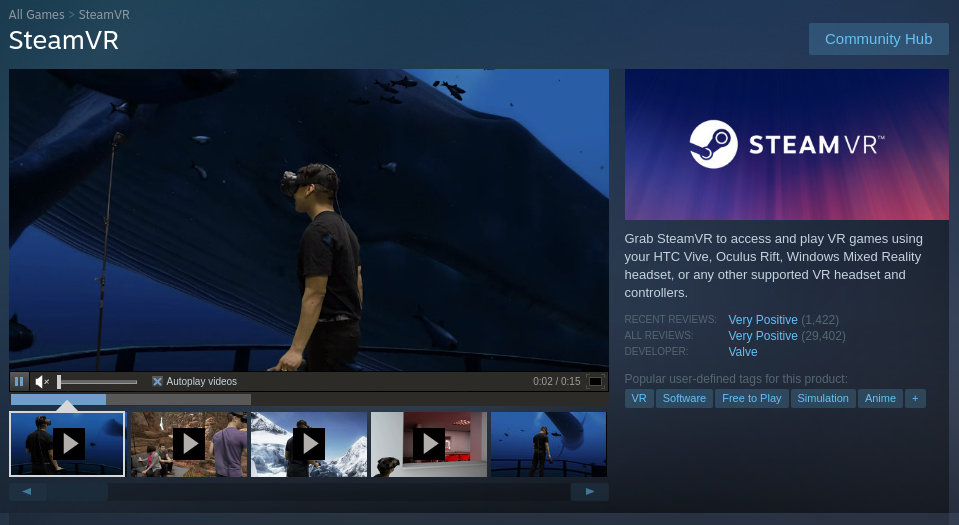
\includegraphics[scale=0.4]{pics/steam-vr-in-store}
    \caption{Steam VR Download}
    \label{fig:steam-vr-in-store}
\end{figure}

Offiziell werden die Valve Index und die HTC Brillen von BeamVR unterstützt.
Somit funktioniert die Applikation mit SteamVR.
Steam VR ist eine Software welche auf Steam herunterladbar ist.
Es ist dabei nicht wichtig, dass die SteamVR Installation vor dem Einstecken der Geräte erfolgt.
Der Download für die Software ist in dem Steam Store zu finden.
In Abb.~\ref{fig:steam-vr-in-store} ist ein Screenshot von der Steam VR Downloadseite zu sehen.

\subsection{VR Headset Verbindung}

Die Verbindung von dem Headset zu dem Computer ist von Headset zu Headset unterschiedlich.
Deshalb wird in Zuge diesr Arbeit nur die Verbindung mit einer HTC Vive Pro beschrieben.
Dabei ist auch die kabellose Variante inkludiert, welche mit dem HTC Vive Wireless Adapter funktioniert.
Für mehr informationen zu dem Adapter wird auf~\ref{subsec:wireless-virtual-reality} verwiesen.

\subsubsection{Tethered}

\begin{figure}
    \centering
    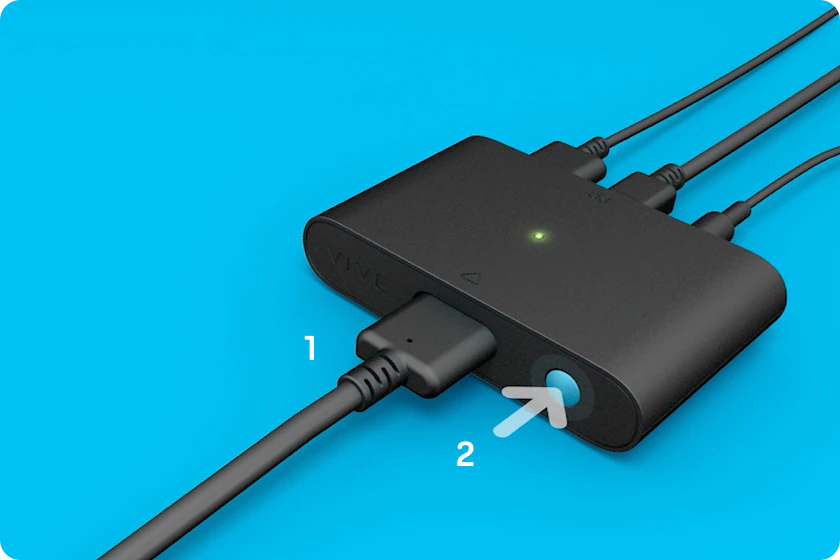
\includegraphics[scale=0.4]{pics/link-box-setup}
    \caption{Aufgesetzte Linkbox}
    \label{fig:link-box-setup}
\end{figure}


In der Box der HTC Vive Pro befindet sich eine sogenannte Linkbox.
Diese Linkbox ist die Zentralstelle, an der das Headset steckt, die Kabel zu dem Computer und das Stromkabel.
Diese Ports sind auf zwei Seiten aufgeteilt.
Eine Seite ist nur für das Headset Kabel und die andere Seite ist für den Strom und die PC-Verbindung.
Das Headset Kabel ist ein spezielles Kabel für die Brille, das Stromkabel ein Power-Adapter und die PC-Verbindung ist ein USB-A Kabel und ein Mini Displayport zu normalen Displayport Kabel~\cite{VivePro_Setup}.
In Abb.~\ref{fig:link-box-setup} ist eine aufgesetzte Linkbox zu sehen.
Für mehr Informationen wird auf~\cite{VivePro_Setup} verwiesen.

\subsubsection{Wireless Adapter}

Mit dem Wireless Adapter kann das Headset ohne Kabel verwendet werden.
Das Aufsetzen von dem Wireless Adapter ist etwas komplizierter.
Wie bereits in dem Abschnitt~\ref{subsec:wireless-virtual-reality} braucht diese Verbindung zu dem Computer auch eine Linkbox.

\begin{figure}
    \centering
    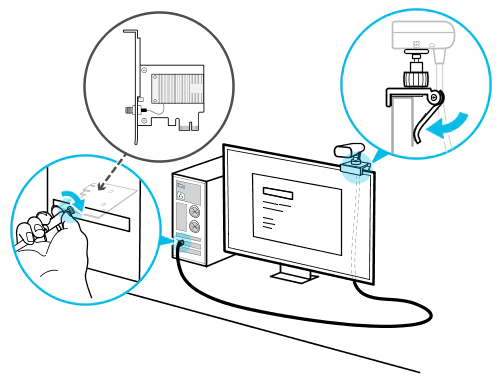
\includegraphics[scale=0.5]{pics/vive-wireless-setup-linkbox}
    \caption{Linkbox Setup~\cite{Wireless_Adapter_Setup_Docs}}
    \label{fig:vive-wireless-setup-linkbox}
\end{figure}


In diesem Fall reicht ein Kabel, welches diese Linkbox verbindet.
Dieses Kabel ist dann mit einer PCIe Karte im Computer verbunden, welche vor diesem Prozess in den Computer eingebaut werden muss.
Die Linkbox an sich muss statisch irgendwo positioniert werden.
Mögliche Orte dafür wären das der Monitor oder die Wand.
Grundsätzlich wäre es optimal, dass die Linkbox eine freie Sicht auf die VR-Brille hat~\cite{Wireless_Adapter_Setup_Docs}.
In Abb.~\ref{fig:vive-wireless-setup-linkbox} ist auf dem Monitor eine mit dem links stehenden PC verbundene Linkbox.

\begin{figure}
    \centering
    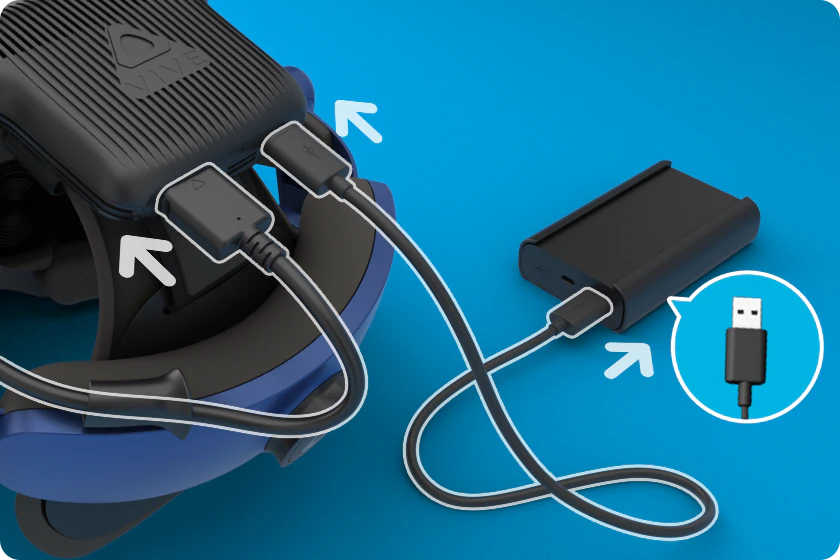
\includegraphics[scale=0.3]{pics/vive-wireless-setup-adapter}
    \caption{Angesteckter Adapter~\cite{Wireless_Adapter_Setup_Page}}
    \label{fig:vive-wireless-setup-adapter}
\end{figure}


Schlussendlich wird für das kabellose Erlebnis noch der Adapter gebraucht, welcher auf die VR-Brille angebracht wird.
Der Adapter besitzt einen Headset kabel Port und einen USB-A Port.
Inkludiert in der Box des Adapters ist ein kürzeres Headset Kabel zur verbindung des Headsets mit dem Adapter.
Der USB-Port wird für die Stromzufuhr gebraucht.
Für den Strom wird eine inkludierte Powerbank mit dem Headset verbunden mittel eines USB-A zu UBS-A Kabel~\cite{Wireless_Adapter_Setup_Page}.
In Abb.~\ref{fig:vive-wireless-setup-adapter} ist ein fertig angesteckter Adapter zu sehen.

Um den Wireless Adapter nun zu verwenden wird noch eine extra Software benötigt, die man von der HTC Vive Seite herunterladen kann.
Mit dieser sollte sich das Headset automatisch mit dem Computer über Steamvr verbinden~\cite{Wireless_Adapter_Setup_Page}.

\subsection{Tracker Verbindung}

Genauso wie die Controller und das Headset funktionieren die Tracker mit der SteamVR Software.
Anders wie bei den Controllern ist die Verbindung zu dem Computer.
Die Verbindung wird über eine Dongle und einer Dongle Halterung gelöst.
Dabei wird die Dongle Halterung an den PC angesteckt und die Dongle in die Dongle Halterung eingesteckt~\cite{vive_tracker_setup_video_2021}.

Sobald die Tracker fertig eingesteckt sind, muss in SteamVR und bei den Trackern die Pairing Modus aktiviert werden.
In Steam VR kann dieser Modus unter \emph{SteamVR Menü > Devices > Pair Controller} gefunden werden.
Der Pairingmodus des Trackers erfolgt mit einem langen drücken des Knopfes in der Mitte des Trackers~\cite{vive_tracker_setup_video_2021}.

\subsection{Steam VR Setup}\label{subsec:steam-vr-setup}

In der SteamVR Applikation kann unter \emph{SteamVR Menü > Room Setup} das Room Setup gefunden werden.
Das Roomsetup ist für die Kalibrierung des Raumes zuständig.
Dies beinhaltet die höhe des Bodens, die Größe des VR Raumes und die Orientierung des VR Raumes.
Bei der BeamVR Applikation ist das Setup ein wichtiger Schritt, um ein immersives Erlebnis zu erreichen.

Zum Zeitpunkt der Erstellung dieser Arbeit konnten keine zuverlässigen Informationen bezüglich des Room Setup gefunden werden.
Trotzdem zeigt sich aus Erfahrung, dass die Kalibrierung des Monitors die initiale Richtung des VR Headsets angibt.
Die Richtung des VR Headsets ist aber auch von dem Seitenverhältnis der VR Fläche abhängig.
Zeigt der Controller bei der Kalibrierung de länge des Raums entlang ist die Orientierung des Headsets trotzdem in Richtung der Breite.
Bedeutet, dass sich die Orientierung in diesem Fall gegen den Uhrzeigersinn um 90 Grad dreht.

\begin{figure}
    \centering
    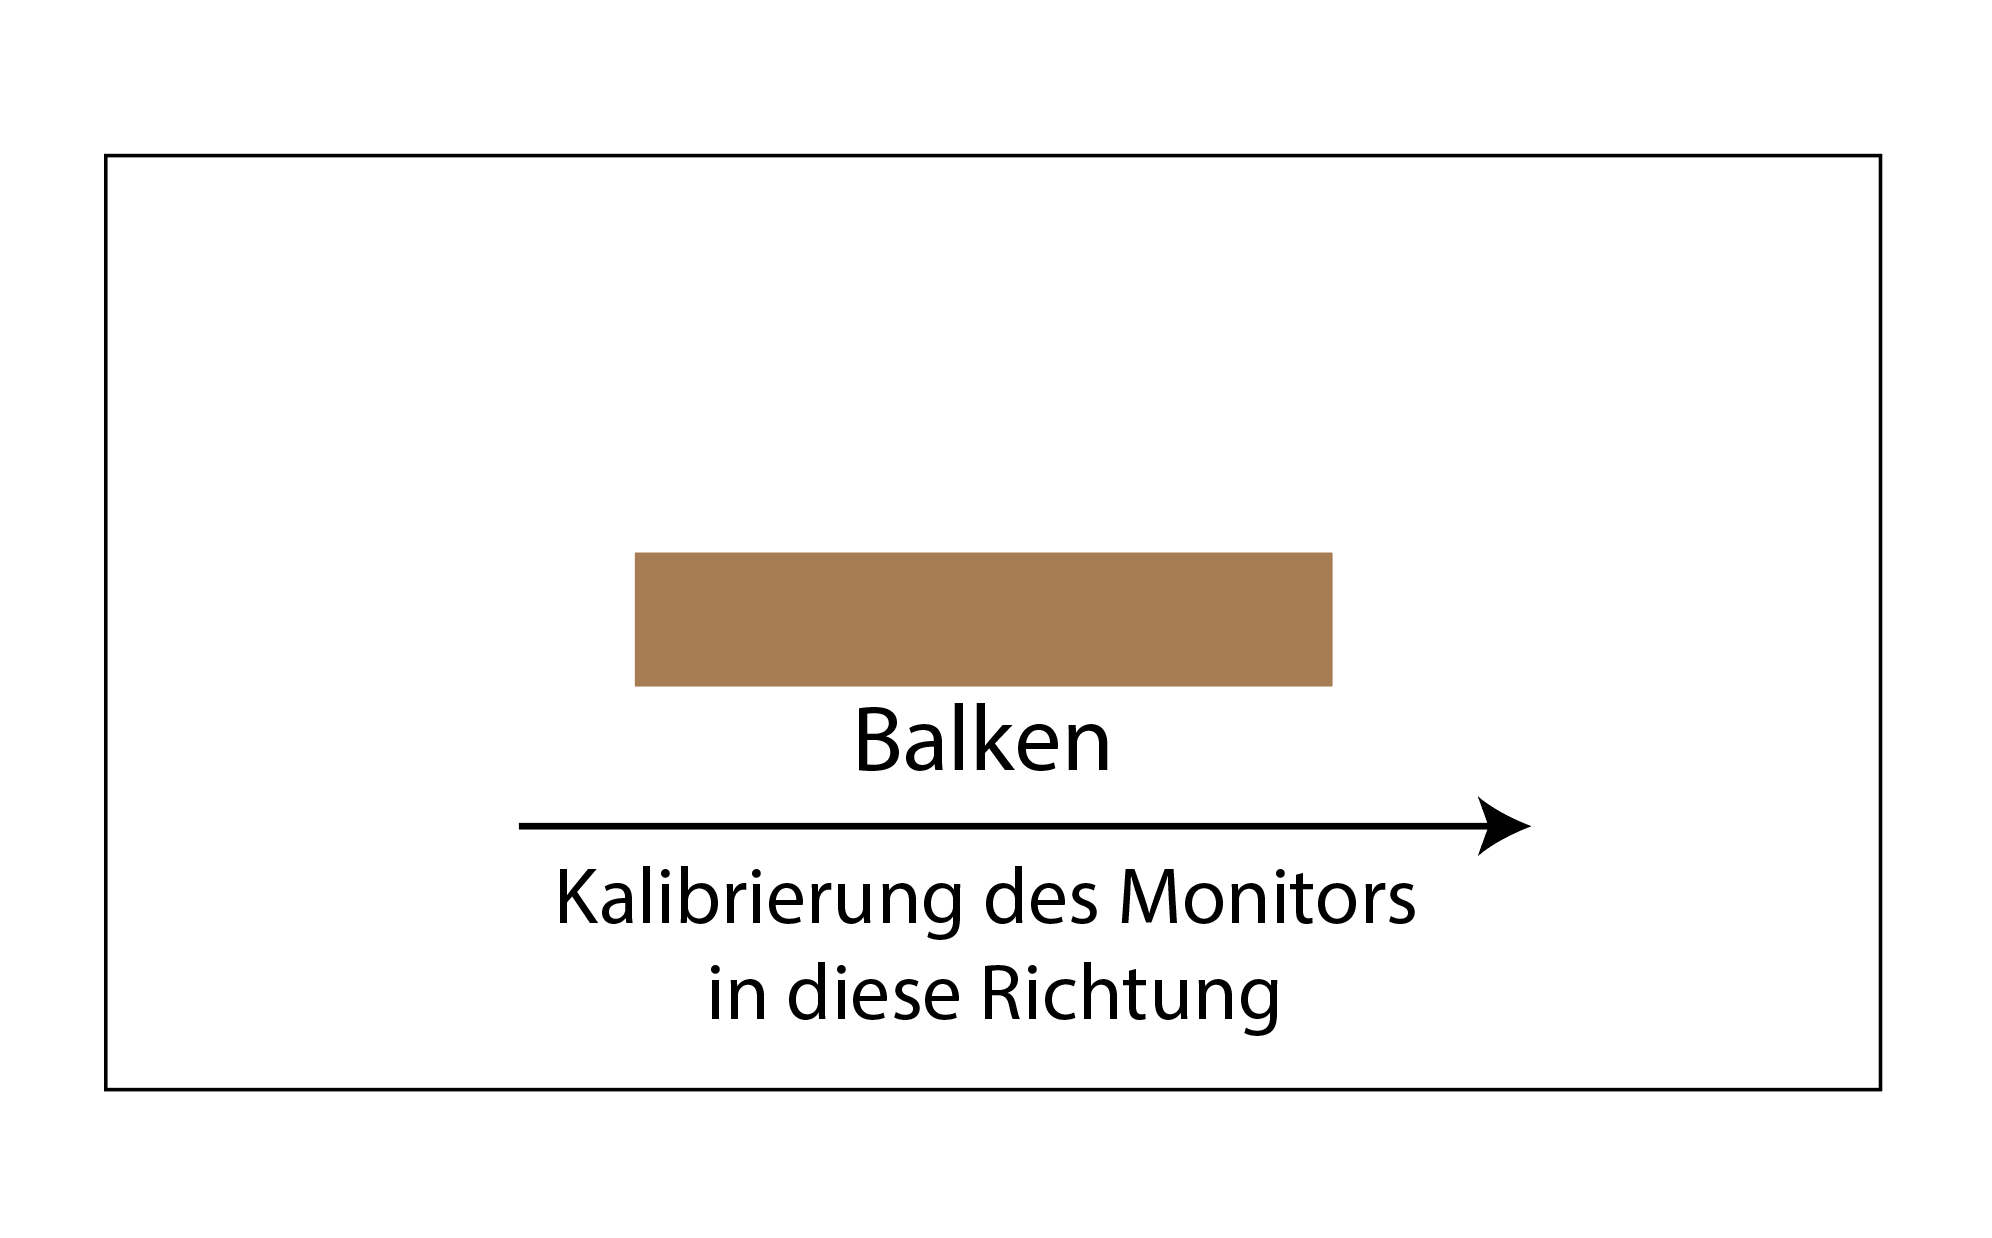
\includegraphics[scale=0.2]{pics/monitor_calibration}
    \caption{Kalibrierung des Monitors und der Maße des VR Raums}
    \label{fig:steam-vr-calibration}
\end{figure}

\begin{figure}
    \centering
    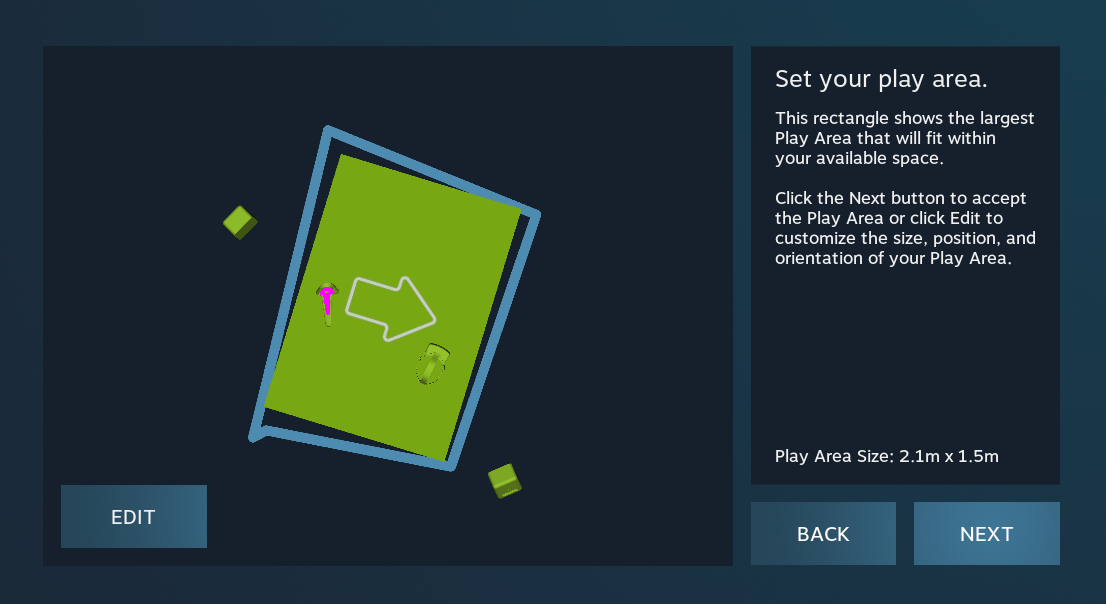
\includegraphics[scale=0.4]{pics/steam-vr-summary}
    \caption{Steam VR Setup Zusammenfassung}
    \label{fig:steam-vr-summary}
\end{figure}



Für BeamVR ist es wichtig, dass die längere Seite in die gleiche Richtung wie der Balken schaut und die kürzere seite in die andere.
Dies ist in Abb.~\ref{fig:steam-vr-calibration} abgebildet.
In der Zusammenfassung des VR Raums sollte die Orientierung wie in Abb.~\ref{fig:steam-vr-summary} ausschauen.

Bei der Kalibrierung des Bodens ist es nur wichtig, dass es möglich genau ist, damit die Gravitation wie erwarted funktioniert.
Für mehr Information über die Gravitaion wird auf~\ref{subsec:gravity} verwiesen.

\subsection{Applikation Starten}\label{subsec:run-application}

Nachdem alles aufgebaut und aufgesetzt ist kann die Applikation in Steam gestartet werden.
Die Applikation kann in dem Unity Editor gestartet werden oder als gebaute Datei.
Wichtig dabei ist, dass das Spiel bei Steam importiert wird, damit das Controller Mapping funktioniert.

\subsection{Beam Kalibration}

Bevor eine der drei Karten ausgewählt werden kann, muss noch die Beam Kalibration stattfinden.
Diese ist für die Ortung des Balkens in der digitalen Welt.
Für mehr Informationen zu der Kalibrierung wird auf den Abschnitt~\ref{subsec:beam-calibration} verwiesen.
Dort wird das Setup noch genauer beschrieben.

\subsection{Full Body Tracking Kalibration}\label{subsec:full-body-tracking-calibration}

\begin{figure}
    \centering
    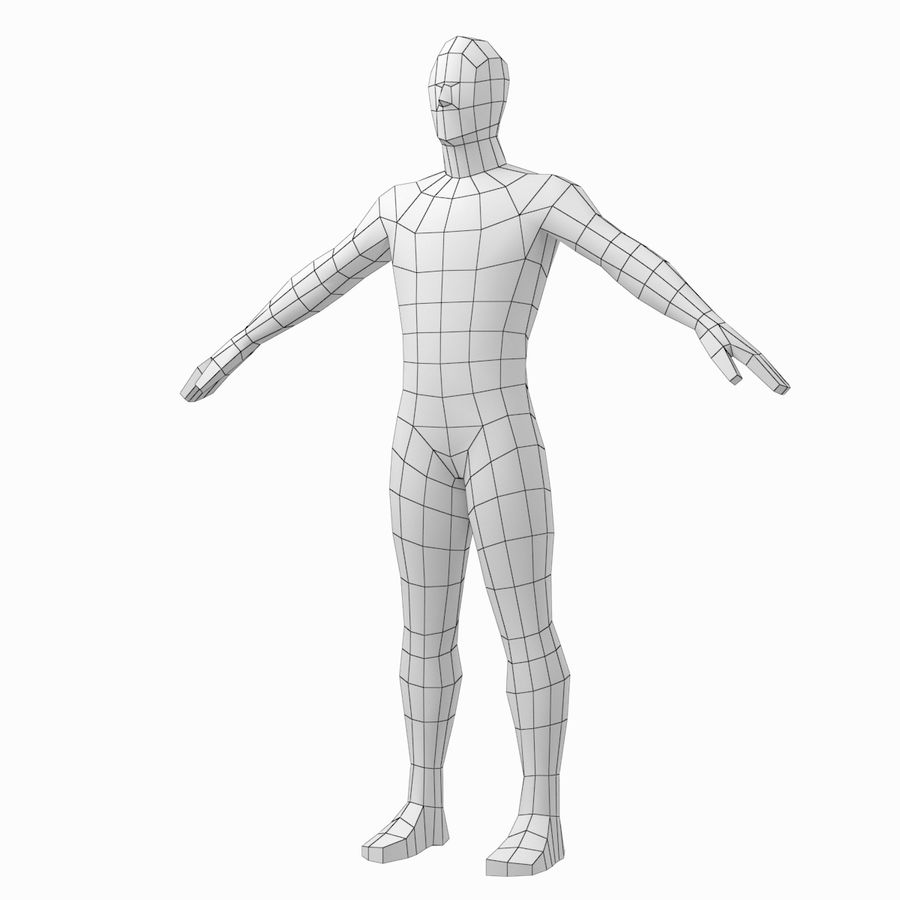
\includegraphics[scale=0.3]{pics/a-pose-human}
    \caption{A-Pose Modell~\cite{vkstudio_2020}}
    \label{fig:a-pose-human}
\end{figure}

\begin{figure}
    \centering
    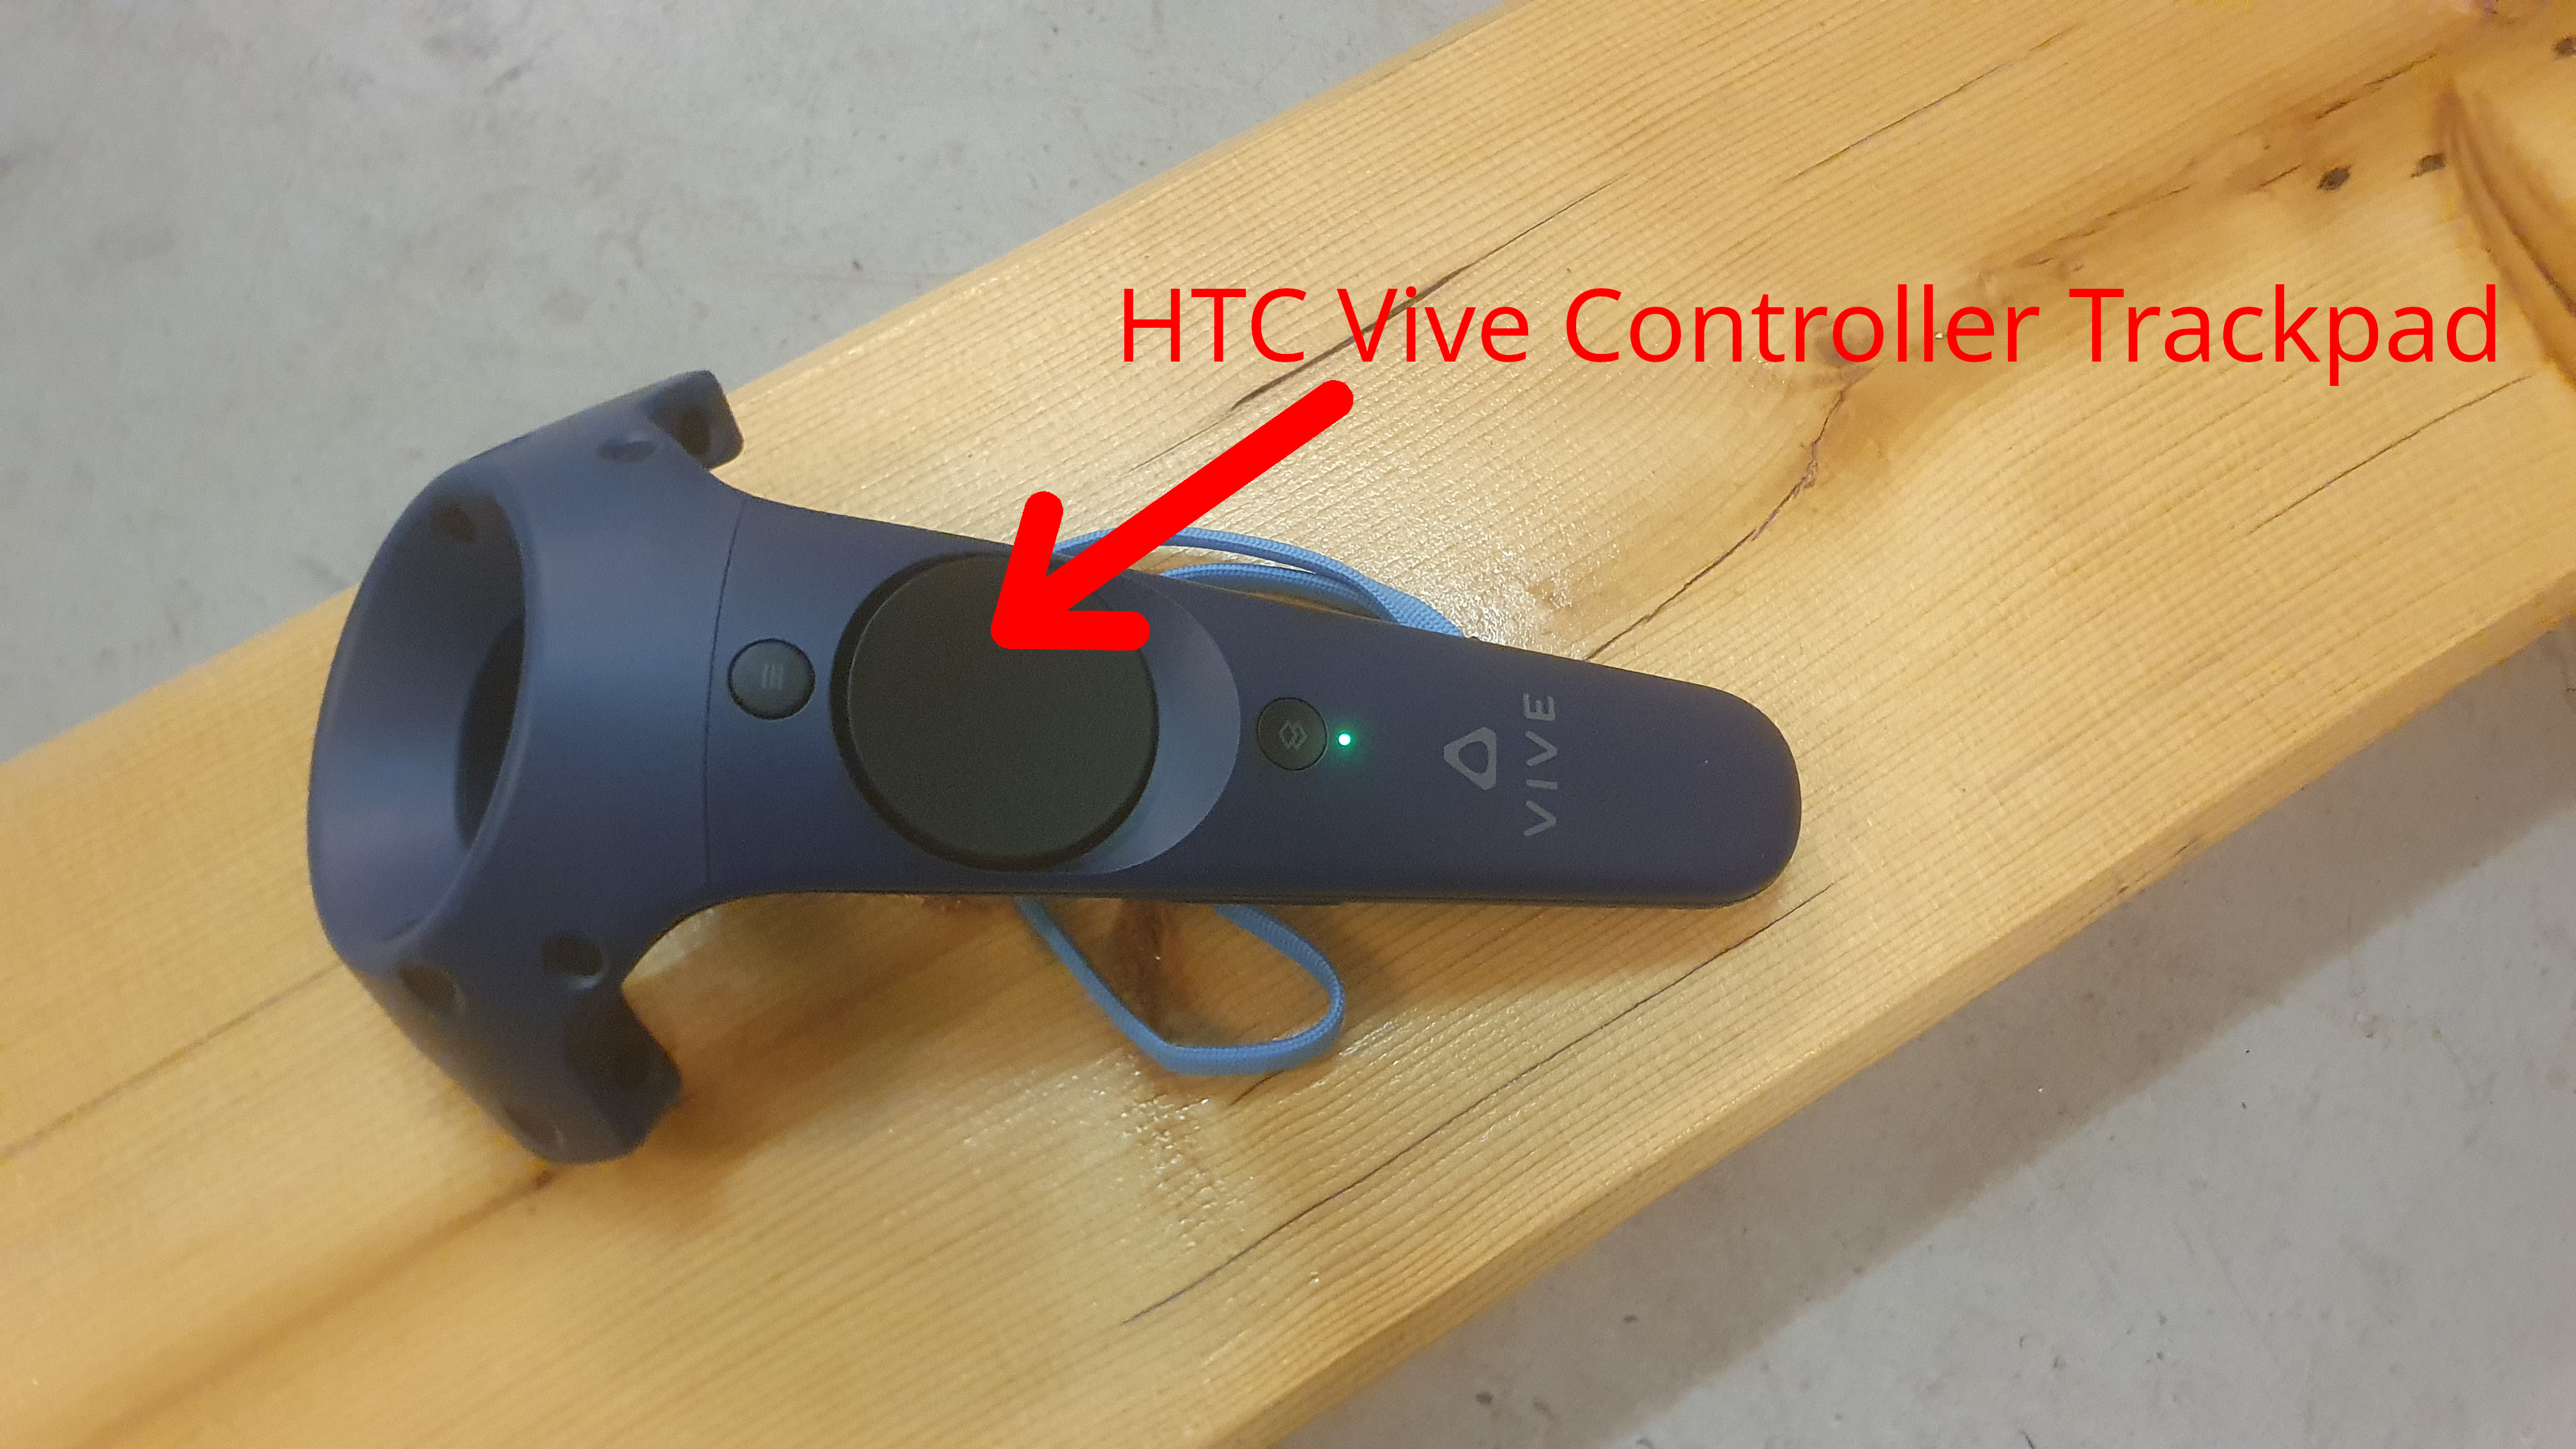
\includegraphics[scale=0.1]{pics/vive_controller_trackpad}
    \caption{Trackpad des HTC Vive Pro Controller}
    \label{fig:vive-controller-trackpad}
\end{figure}



Nach der Beam Kalibration ist es möglich eine Karte auszuwählen.
In diesen Karten steht vorne am Balken ein Spieler Modell.
Das Full Body Tracking wird durch Drücken des Trackpads auf dem Controllers aktiviert.
In Abb.~\ref{fig:vive-controller-trackpad} ist das Trackpad eines HTC Vive Controller zu sehen.

Für ein gutes Tracking sollte eine möglichst natürliche Pose, wie beispielsweise eine A-Pose, eingehalten werden.
Diese A-Pose ist in Abb.~\ref{fig:a-pose-human} abgebildet.

